%%%%%%%%%%%%%%%%%%%%%%%%%%%%%%%%%%%%%%%%%%%%%%%%%%%%%%%%%%%%%%%%%%%%%%
% Lớp 10 | Mệnh đề. Tập hợp | Mệnh đề
% Dạng 0D1?1-2: Tính đúng-sai của mệnh đề
% Số câu: 135  (sinh tự động bởi tach_cau.py; từ nay thầy sửa trực tiếp file này)
%%%%%%%%%%%%%%%%%%%%%%%%%%%%%%%%%%%%%%%%%%%%%%%%%%%%%%%%%%%%%%%%%%%%%%

%%%%%%%%%%%%%%%% TRẮC NGHIỆM 4 PHƯƠNG ÁN %%%%%%%%%%%%%%%%

% nguồn: MaHoaNH_TracNghiem_Lop10
\begin{ex}%[0D1N1-2]%[ma:0f81d379]
	Cho $P(x)\colon$\lq\lq$2x-1>0$\rq\rq. Với $x$ là số tự nhiên. Mệnh đề nào sau đây  đúng?
	\choice {\True  $P(1)$}{ $P(0)$}{ $P(-1)$}{ $P(-2)$}
	\loigiai{ 
		Với $x$ là số  tự nhiên, ta có $x\in\{0;1;2;\ldots\}$.\\
		$x=1$ thì $P(1)\colon 2\cdot1-1>0 \Leftrightarrow 1>0$ là một mệnh  đề đúng.
	} 
\end{ex}

% nguồn: MaHoaNH_TracNghiem_Lop10
\begin{ex}%[0D1N1-2]%[ma:14ffef94]
	 Mệnh đề nào sau đây là mệnh đề đúng?
	 \choice
		{Tứ giác có 4 cạnh bằng nhau là  hình vuông}
		{Tứ giác có 2 đường chéo bằng  nhau là hình chữ nhật}
		{\True Hình thang cân có 1  góc vuông là hình chữ nhật}
		{Hình thoi là hình vuông có 1 góc  vuông}
	\loigiai{ 
	 }
\end{ex}

% nguồn: MaHoaNH_TracNghiem_Lop10
\begin{ex}%[0D1N1-2]%[ma:68092957]
	Mệnh đề nào sau đây  là mệnh đề \textbf{sai}?
	\choice  {\True $\forall x\in\mathbb{R}\colon x^{2}>0"$}{$"\exists n\in\mathbb{N}\colon n=n^{2"}$}{$"\exists n\in\mathbb{N}\colon n\le2n"$}{$"\exists x\in\mathbb{R}\colon x>x^2"$}
	 \loigiai{
		Ta có $x^{2}\ge0$, $\forall x\in\mathbb{R}$ (vì với $x=0$  thì $x^2=0$, không lớn hơn $0$).\\
		Vì tồn tại $n=1$ thỏa  mãn ($1=1^2$).\\
		Vì tồn tại $n=1$  thỏa mãn ($1\le2\cdot1$).\\
		vì tồn tại  $x=\dfrac{1}{2}$ thỏa mãn ($\dfrac{1}{2}>(\dfrac{1}{2})^2=\dfrac{1}{4}$).
	} 
\end{ex}

% nguồn: MaHoaNH_TracNghiem_Lop10
\begin{ex}%[0D1N1-2]%[ma:6a11339f]
	 Cho $x$ là một phần tử của tập hợp $X$. Mệnh đề nào sau đây là $\textbf{đúng}$?
	 \choice
		 {\True $x \in X$}
		{$X  \in x$}
		 {$x \subset X$}
		{$\{x\} \in X$} 
	\loigiai{ 
		Mệnh đề là đúng là $x \in X$. Kí hiệu $x$ là một phần  tử của tập hợp $X$.
	 }
\end{ex}

% nguồn: MaHoaNH_TracNghiem_Lop10
\begin{ex}%[0D1N1-2]%[ma:d239a812]
	Khẳng định nào sau đây là mệnh đề toán  học?
	 \choice
		{\True $4$ là một số  chẵn}
		{Số  $x$ nhỏ hơn $1$}
		{Cơn bão Yagi để lại hậu quả nặng nề  quá!}
		{Học hành tiến  bộ nhé!}
	 \loigiai{
		$4$ là một số chẵn  là mệnh đề toán học.
	 }
\end{ex}

% nguồn: MaHoaNH_TracNghiem_Lop10
\begin{ex}%[0D1N1-2]%[ma:906bc6e5]
	Trong các mệnh đề sau có bao nhiêu  mệnh đề \textbf{sai}?
	\begin{enumerate}
		\item $3\ge3$; 
		\item $\forall x\in\mathbb{R}:x^{2}>0$; 
		\item $10-2+4=4$; 
		 \item $1<-3$.
	\end{enumerate}
	\choice {\True $3$}{$1$}{$2$}{$4$} 
	\loigiai{ 
		Mệnh để $3\ge3$  đúng.\\
		 Vậy có 3 mệnh đề sai.
	} 
\end{ex}

% nguồn: MaHoaNH_TracNghiem_Lop10
\begin{ex}%[0D1N1-2]%[ma:0f915a99]
	Cho tứ giác $ABCD$ có $\overrightarrow{AD}=\overrightarrow{BC}$. Mệnh đề nào trong các mệnh  đề sau là \textbf{sai}?
	 \choice
		{Tứ  giác $ABCD$ là hình bình hành}
		{$DA=BC$} 
		{\True $\overrightarrow{AC}=\overrightarrow{BD}$} 
		 {$\overrightarrow{AB}=\overrightarrow{DC}$}
	 \loigiai{
	\immini 
		{$AC$ và $BD$ là hai đường chéo của tứ giác $ABCD$ nên hai vectơ $\overrightarrow{AC}$, $\overrightarrow{BD}$ không cùng phương  vì vậy không thể bằng nhau.}
		 {
		\begin{tikzpicture}[scale=1,line join=round,line cap=round,font=\footnotesize,>=stealth]
				 \def\d{4}
				\def\r{3} 
				\path (0:0) coordinate (B) 
					++(0:\d)  coordinate (C)
					++(50:\r) coordinate (D) 
					($(B)+(D)-(C)$) coordinate (A); 
				 \draw (A)--(B)--(C)--(D)--cycle;
				\foreach \x/ \goc  in {A/180,B/180,C/0,D/0}
				\fill (\x) circle (1pt) 
					 ($(\x)+(\goc:3mm)$) node {$\x$};
			\end{tikzpicture}
		 }
	 }
\end{ex}

% nguồn: MaHoaNH_TracNghiem_Lop10
\begin{ex}%[0D1N1-2]%[ma:2a121e78]
	Gọi $O$ là giao điểm hai  đường chéo $AC$ và $BD$ của hình bình hành $ABCD$. Đẳng thức nào sau đây là đẳng thức \textbf{sai}?
	\choice 
		{$\overrightarrow{OB}=\overrightarrow{DO}$} 
		 {$\overrightarrow{AB}=\overrightarrow{DC}$}
		{\True  $\overrightarrow{OA}=\overrightarrow{OC}$}
		 {$\overrightarrow{CB}=\overrightarrow{DA}$}
	\loigiai{ 
	 \immini
		{$\overrightarrow{OA}$ và $\overrightarrow{OC}$ là hai vectơ đối nhau nên  không thể bằng nhau.}
		{ 
		\begin{tikzpicture}[scale=1,line join=round,line cap=round,font=\footnotesize,>=stealth]
				 \def\d{4}
				\def\r{3} 
				\path  (0:0) coordinate (B)
					++(0:\d) coordinate (C) 
					 ++(50:\r) coordinate (D)
					 ($(B)+(D)-(C)$) coordinate (A)
					(intersection  of A--C and B--D) coordinate (O);
				\draw  (A)--(B)--(C)--(D)--cycle (A)--(C)
					(B)--(D); 
				\foreach \x/ \goc in  {A/180,B/180,C/0,D/0,O/80}
				\fill (\x) circle  (1pt)
					($(\x)+(\goc:3mm)$)  node {$\x$};
			\end{tikzpicture}
		} 
	 }
\end{ex}

% nguồn: MaHoaNH_TracNghiem_Lop10
\begin{ex}%[0D1N1-2]%[ma:2c0bbf3d]
	Cho hình lục giác đều $ABCDEF$ tâm $O$. Số các vectơ khác vectơ không, cùng phương với vectơ $\overrightarrow{OB}$ có điểm đầu và điểm cuối là các đỉnh của lục giác  là
	\choice 
		{$4$} 
		{\True  $6$}
		{$8$} 
		{$10$} 
	 \loigiai{
		\begin{center}
			\begin{tikzpicture}[scale=1,line join=round,line cap=round,font=\footnotesize,>=stealth]
					\def\a{2} 
					\path (0:0) coordinate  (O)
						(0:\a) coordinate (C) 
						(60:\a) coordinate (D) 
						(120:\a)  coordinate (E)
						(180:\a)  coordinate (F)
						(240:\a)  coordinate (A)
						(300:\a)  coordinate (B);
					\draw  (A)--(B)--(C)--(D)--(E)--(F)--(A)
						(O)--(B); 
					\foreach \x/  \goc in {A/180,B/-135,C/-45,D/0,E/90,F/180,O/0}
					\fill (\x) circle (1pt) 
						 ($(\x)+(\goc:3mm)$) node {$\x$};
				\end{tikzpicture}
		\end{center}
		Các vectơ cùng  phương với vectơ $\overrightarrow{OB}$ là\\
		$\overrightarrow{BE}$, $\overrightarrow{EB}$,  $\overrightarrow{DC}$, $\overrightarrow{CD}$, $\overrightarrow{FA}$, $\overrightarrow{AF}$.
	} 
\end{ex}

% nguồn: MaHoaNH_TracNghiem_Lop10
\begin{ex}%[0D1N1-2]%[ma:3ec830f8]
	Cho  hình bình hành $ABCD$ tâm $O$. Gọi $P$, $Q$, $R$ lần lượt là trung điểm của $AB$, $BC$, $AD$. Tìm mệnh đề \textbf{sai}.
	 \choice
		{Có $2$ vectơ bằng  $\overrightarrow{PR}$}
		 {Có $4$ vectơ bằng $\overrightarrow{AR}$}
		{Có $2$ vectơ  bằng $\overrightarrow{BO}$}
		{\True Có $5$ vectơ  bằng $\overrightarrow{OP}$}
	\loigiai{ 
	 \immini
		 {Ta có
		\begin{eqnarray*}
			 &&\overrightarrow{PQ}=\overrightarrow{AO}=\overrightarrow{OC}.\\
			&&\overrightarrow{AR}=\overrightarrow{RD}=\overrightarrow{PO}=\overrightarrow{BQ}=\overrightarrow{QC}.\\ 
			 &&\overrightarrow{BO}=\overrightarrow{OD}=\overrightarrow{PR}.\\
			 &&\overrightarrow{OP}=\overrightarrow{RA}=\overrightarrow{DR}=\overrightarrow{CQ}=\overrightarrow{QB}.
		\end{eqnarray*}}
		 {
		\begin{tikzpicture}[scale=1,line join=round,line cap=round,font=\footnotesize,>=stealth]
				\def\d{4} 
				\def\r{3} 
				 \path (0:0) coordinate (B)
					++(0:\d) coordinate  (C)
					 ++(50:\r) coordinate (D)
					($(B)+(D)-(C)$) coordinate  (A)
					(intersection of A--C and B--D) coordinate  (O)
					($(A)!0.5!(B)$) coordinate (P) 
					 ($(B)!0.5!(C)$) coordinate (Q)
					($(A)!0.5!(D)$)  coordinate (R);
				\draw (A)--(B)--(C)--(D)--cycle (A)--(C) 
					 (B)--(D)
					 (P)--(R)
					 (O)--(P);
				\foreach \x/ \goc in  {A/180,B/180,C/0,D/0,O/80,P/180,Q/-90,R/90}
				\fill  (\x) circle (1pt)
					($(\x)+(\goc:3mm)$)  node {$\x$};
			\end{tikzpicture}
		} 
	 }
\end{ex}

% nguồn: MaHoaNH_TracNghiem_Lop10
\begin{ex}%[0D1H1-2]%[ma:7268d2e7]
	Tìm  mệnh đề đúng.
	\choice {Điều kiện cần và đủ để một số tự nhiên chia hết cho 15 là số đó chia hết cho 5}{\True Điều kiện đủ để ít nhất một trong hai số $a, b$ là số dương là $a+b>0$}{Điều kiện cần và đủ để tứ giác là hình chữ nhật là nó có hai đường chéo  bằng nhau}{Điều kiện cần và đủ để $a$ và $b$ đều là số hữu tỉ là $a+b$ là số hữu tỉ}
	 \loigiai{
		Ta có $a+b>0$ thì ít nhất một trong hai số $a, b$ là số dương. Đây là mệnh đề đúng nên điều kiện đủ để ít nhất một trong hai số $a, b$  là số dương là $a+b>0$.
	 }
\end{ex}

% nguồn: MaHoaNH_TracNghiem_Lop10
\begin{ex}%[0D1H1-2]%[ma:5599ea82]
	Tìm mệnh đề  đúng.
	 \choice {\True \lq\lq$\forall n\in\mathbb{N}\colon n(n+1)(n+2)$ chia hết cho $6$\rq\rq}{\lq\lq$\forall n\in\mathbb{N}\colon n^{2}+1$ là số lẻ\rq\rq}{\lq\lq $\exists x\in\mathbb{R}\colon x^{2}<0$\rq\rq}{\lq\lq$\forall x\in\mathbb{R}\colon x^{2}=x$\rq\rq}
	 \loigiai{
		\lq\lq$\forall n\in\mathbb{N}\colon n(n+1)(n+2)$ chia hết cho $6$\rq\rq~ đúng vì $n(n+1)(n+2)$ là tích 3 số tự nhiên  liên tiếp nên chia hết cho 6.\\
		\lq\lq$\forall n\in\mathbb{N}\colon n^{2}+1$ là số lẻ\rq\rq~ sai vì với $n=3$ thì $n^{2}+1=10$  là số chẵn.\\
		\lq\lq $\exists x\in\mathbb{R}\colon x^{2}<0$\rq\rq sai  vì $x^{2}\ge0$, $\forall x\in\mathbb{R}$.\\
		\lq\lq$\forall  x\in\mathbb{R}\colon x^{2}=x$\rq\rq~ sai vì với $x=2$ thì $x^{2}\ne x$.
	} 
\end{ex}

% nguồn: MaHoaNH_TracNghiem_Lop10
\begin{ex}%[0D1H1-2]%[ma:3bc00a9c]
	Trong các mệnh  đề sau tìm mệnh đề \textbf{đúng}?
	\choice 
		{$\forall x \in \mathbb{R}$,  $ x^2>0$}
		{$\forall x \in  \mathbb{N}$, $ x\vdots 3$}
		{$\forall  x \in \mathbb{R}$, $-x^2<0$}
		{\True $\exists x \in \mathbb{R}$, $ x>x^2$} 
	\loigiai{ 
		Mệnh đề $\exists x  \in \mathbb{R}$, $ x>x^2$ là đúng. Vì $\exists 0{,}5 \in \mathbb{R}$, $ 0{,}5>0{,}5^2$.
	 }
\end{ex}

% nguồn: MaHoaNH_TracNghiem_Lop10
\begin{ex}%[0D1H1-2]%[ma:eab968eb]
	Trong các  mệnh đề sau, mệnh đề nào \textbf{đúng}?
	 \choice
		{$6 \sqrt{2}$  là số hữu tỷ}
		{\True Phương trình $x^2+7x-2=0$ có $2$  nghiệm trái dấu}
		{$17$ là số  chẵn}
		{Phương trình $x^2+x+7=0$  có nghiệm}
	 \loigiai{
		Phương trình $x^2+7x-2=0$ có  $a\cdot c=-2<0$ nên phương trình có $2$ nghiệm trái dấu.
	} 
\end{ex}

% nguồn: MaHoaNH_TracNghiem_Lop10
\begin{ex}%[0D1H1-2]%[ma:6085fbfd]
	Chọn mệnh đề \textbf{đúng} trong các mệnh đề sau 
	 \choice
		{\True $\forall  x\in \mathbb{R}$, $x+1 > x$}
		{$\forall x\in  \mathbb{R}$, $\left| x\right|=x$}
		{$\exists  x\in \mathbb{R}$, $x-3=x^2$}
		 {$\exists x\in \mathbb{R}$, $x^2< 0$}
	 \loigiai{
		Mệnh đề  $\forall x\in \mathbb{R}$, $x+1 > x$ luôn đúng.
	 }
\end{ex}

% nguồn: MaHoaNH_TracNghiem_Lop10
\begin{ex}%[0D1H1-2]%[ma:d1039a2e]
	Mệnh đề nào sau  là mệnh đề \textbf{sai}?
	\choice 
		{$\forall n \in \mathbb{N} $, $ n  \leq 2 n$}
		{$\exists  n \in \mathbb{N} $, $ n^2=n$}
		{\True $\forall x  \in \mathbb{R}$, $ x^2>0$}
		{$\exists x \in  \mathbb{R}$, $ x>x^2$}
	 \loigiai{
		Mệnh đề $\forall x \in \mathbb{R}$, $ x^2>0$ là \textbf{sai}.  Vì $\exists 0 \in \mathbb{R}$, $ 0^2=0$.
	} 
\end{ex}

% nguồn: MaHoaNH_TracNghiem_Lop10
\begin{ex}%[0D1H1-2]%[ma:544e29ce]
	Trong các mệnh đề dưới đây mệnh đề  nào \textbf{đúng}?
	 \choice
		 {\True $\forall x \in \mathbb{R}$, $x^2+1>0$}
		{$\forall x \in \mathbb{R}$,  $x^2>x$}
		 {$\exists r \in \mathbb{Q}$, $r^2=7$}
		 {$\forall n \in \mathbb{N}$, $n+4$ chia hết cho $4$}
	\loigiai{ 
		Mệnh  đề $\forall x \in \mathbb{R}$, $x^2+1>0$ luôn đúng.
	 }
\end{ex}

% nguồn: MaHoaNH_TracNghiem_Lop10
\begin{ex}%[0D1H1-2]%[ma:e93fafb8]
	Cho $n$ là số  tự nhiên, mệnh đề nào sau đây \textbf{đúng}?
	 \choice
		{$\forall n$, $n\left(n+1\right)$ là số chính  phương}
		{$\forall n$, $n\left(n+1\right)$ là  số lẻ}
		{$\exists n$, $n\left(n+1\right)\left(n+2\right)$ là  số lẻ}
		{\True $\forall n$,  $n\left(n+1\right)\left(n+2\right)$ là số chia hết cho $6$}
	 \loigiai{
		Mệnh đề $\forall n$, $n\left(n+1\right)\left(n+2\right)$ là tích của $3$ số tự nhiên liên tiếp, trong đó luôn có một số chia hết cho $2$ và một số  chia hết cho $3$ nên nó chia hết cho $2\cdot3=6$.
	} 
\end{ex}

% nguồn: MaHoaNH_TracNghiem_Lop10
\begin{ex}%[0D1H1-2]%[ma:5f7cfafc]
	Cho các mệnh đề  sau, mệnh đề nào là đúng?
	 \choice
		 {\lq\lq $\exists x\in \mathbb{Z}, 2x^2-3x-4=0$\rq\rq}
		{\True \lq\lq $\forall x\in \mathbb{R}, x^2+x+1> 0$\rq\rq} 
		{\lq\lq $\forall x\in  \mathbb{R}, x^2-4=0$\rq\rq}
		{\lq\lq $\exists x\in \mathbb{N}, x^2-x  < 0$\rq\rq}
	\loigiai{ 
		Ta có \lq\lq $\forall x\in  \mathbb{R}, x^2+x+1> 0$\rq\rq\, là mệnh đề đúng vì $x^2+x+1=\left(x+\dfrac{1}{2} \right)^2+\dfrac{3}{4} > 0, \forall x\in \mathbb{R}$.
	} 
\end{ex}

% nguồn: MaHoaNH_TracNghiem_Lop10
\begin{ex}%[0D1H1-2]%[ma:03d7a8ae]
	Hỏi  trong các mệnh đề sau đây mệnh đề nào là mệnh đề \textbf{đúng}?
	\choice 
		{\True $\forall x  \in \mathbb{R}$, $x>3 \Rightarrow x^2>9$}
		{$\forall  x \in \mathbb{R}$, $x>-3 \Rightarrow x^2>9$}
		{$\forall x \in  \mathbb{R}$, $x^2>9 \Rightarrow x>3$}
		{$\forall x \in \mathbb{R}$,  $x^2>9 \Rightarrow x>-3$}
	\loigiai{ 
		Ta có \lq\lq$\forall x \in \mathbb{R}$, $x>3 \Rightarrow x^2>9$\rq\rq 
		\, là mệnh đề \textbf{đúng}. 
	} 
\end{ex}

% nguồn: MaHoaNH_TracNghiem_Lop10
\begin{ex}%[0D1H1-2]%[ma:52ff7c97]
	Cho đường  tròn tâm $O$. Từ điểm $A$ nằm ngoài $(O)$, kẻ hai tiếp tuyến $AB$, $AC$ tới $(O)$.\\
	 Xét mệnh đề:\\
	 (I) $\overrightarrow{AB}=\overrightarrow{AC}$\\
	(II) $\overrightarrow{OB}=-\overrightarrow{OC}$\\ 
	(III)  $\left|\overrightarrow{BO}\right|=\left|\overrightarrow{CO}\right|$\\
	Mệnh đề \textbf{đúng} là: 
	 \choice
		{Chỉ (I)} 
		 {(I) và (III)}
		 {(I), (II), (III)}
		{\True Chỉ  (III)}
	\loigiai{ 
		Ta có $OB=OC=R\Rightarrow\left|\overrightarrow{BO}\right|=\left|\overrightarrow{CO}\right|$. 
	 }
\end{ex}

% nguồn: MaHoaNH_TracNghiem_Lop10
\begin{ex}%[0D1H1-2]%[ma:50b95212]
	Cho tam giác $ABC$ có $H$ là trực tâm và $O$ là tâm đường tròn ngoại tiếp. Gọi $D$ là điểm đối xứng với $B$ qua $O$. Chọn mệnh đề đúng trong các mệnh đề sau? 
	 \choice
		{\True  $\overrightarrow{AH}=\overrightarrow{DC}$}
		 {$\overrightarrow{AB}=\overrightarrow{DC}$}
		 {$\overrightarrow{AD}=\overrightarrow{BC}$}
		 {$\overrightarrow{AO}=\overrightarrow{AH}$}
	\loigiai{\begin{center}
		\begin{tikzpicture}[line join=round,line cap = round,>=stealth,scale=.8,font=\footnotesize,transform shape]
				 \foreach \x/\y/\z/\g in
					{ 
					0/0/O/170,-2/3/B/90,3/-2/C/-45,-3/-2/A/-135,2/-3/D/-90,-2/-1/H/135 
				} 
				\draw[fill=black]  (\x,\y) circle (1pt) coordinate (\z)
					($(\z)+(\g:3.5mm)$) node{$\z$}; 
				 \pgfmathsetmacro\rr{sqrt (13)}
				 \draw (B)--(A)--(D)--(C)--(B)--(H)--(D)--(B)
					(H)--(A)--(C)--(H); 
				\draw (O) circle  (\rr);
			\end{tikzpicture}
	\end{center}
	Ta có thể chỉ ra được $ADCH$ là hình  bình hành $\Rightarrow\overrightarrow{AH}=\overrightarrow{DC}$.
} 
\end{ex}

% nguồn: MaHoaNH_TracNghiem_Lop10
\begin{ex}%[0D1H1-2]%[ma:2e1e8422]
	Cho hình chữ nhật $ABCD$ có $AB=3$, $BC=4$.  Tính độ dài của vectơ $\overrightarrow{CA}$.
	\choice 
		{\True $\left|\overrightarrow{CA}\right|=5$} 
		{$\left|\overrightarrow{CA}\right|=25$} 
		{$\left|\overrightarrow{CA}\right|=7$} 
		{$\left|\overrightarrow{CA}\right|=\sqrt  7 $}
	\loigiai{ 
	\immini 
		{Xét tam giác $ABC$ vuông tại  $B$, ta có\\ $\left|\overrightarrow{CA}\right|=CA=\sqrt{AB^2+BC^2}=5$.}
		{ 
		\begin{tikzpicture}[scale=1,line join=round,line cap=round,font=\footnotesize,>=stealth]
				\def\d{4} 
				 \def\r{3}
				 \path (0:0) coordinate (B)
					++(0:\d) coordinate  (C)
					++(90:\r) coordinate (D) 
					++(180:\d) coordinate (A); 
				 \draw (A)--(B)--(C)--(D)--cycle (C)--(A);
				 \foreach \x/ \goc in {A/135,B/-135,C/-45,D/45}
				\fill  (\x) circle (1pt)
					 ($(\x)+(\goc:3mm)$) node {$\x$};
			\end{tikzpicture}
		} 
	} 
\end{ex}

% nguồn: MaHoaNH_TracNghiem_Lop10
\begin{ex}%[0D1H1-2]%[ma:0672b2d1]
	Cho  tam giác $ABC$ đều cạnh $2a$. Gọi $M$ là trung điểm $BC$. Khi đó $\left|\overrightarrow{AM}\right|$ bằng
	\choice 
		 {$2a$}
		{$2a\sqrt 3 $} 
		{$4a$} 
		{\True $a\sqrt 3  $}
	 \loigiai{
	\immini 
		{Xét tam  giác $ABM$ vuông tại $M$, ta có\\ $\left|\overrightarrow{AM}\right|=AM=\sqrt{A{B^2}-B{M^2}}\\
		 =\sqrt{(2a)^2-a^2}\\
		 =a\sqrt 3$.}
		{ 
		\begin{tikzpicture}[scale=1,line join=round,line cap=round,font=\footnotesize,>=stealth]
				\def\a{3} 
				\path  (0:0) coordinate (B)
					++(0:\a)  coordinate (C)
					 ([turn]120:\a) coordinate (A)
					 ($(B)!0.5!(C)$) coordinate (M);
				\draw  (A)--(B)--(C)--cycle;
				\foreach \x/  \goc in {A/135,B/-135,C/-45,M/-90}
				 \fill (\x) circle (1pt)
					($(\x)+(\goc:3mm)$) node {$\x$}; 
			\end{tikzpicture}
		} 
	 }
\end{ex}

% nguồn: MaHoaNH_TracNghiem_Lop10
\begin{ex}%[0D1H1-2]%[ma:d4ac1134]
	Cho hình thoi $ABCD$ tâm $O$, cạnh bằng $a$ và $\widehat A=60^\circ $. Kết luận nào sau đây là  \textbf{đúng}?
	\choice 
		 {\True $\left|\overrightarrow{AO}\right|=\dfrac{a\sqrt 3}{2}$}
		{$\left|\overrightarrow{OA}\right|=a$} 
		 {$\left|\overrightarrow{OA}\right|=\left|\overrightarrow{OB}\right|$}
		{$\left|\overrightarrow{OA}\right|=\dfrac{a\sqrt  2}{2}$}
	\loigiai{ 
	 \immini
		{Vì $\widehat A=60^\circ\Rightarrow\Delta ABD$ đều  $\Rightarrow AO=\dfrac{a\sqrt 3}{2}\Rightarrow\left|\overrightarrow{AO}\right|=\dfrac{a\sqrt3}{2}$.}
		 {
		\begin{tikzpicture}[scale=1,line join=round,line cap=round,font=\footnotesize,>=stealth]
				 \def\a{3}
				 \path (0:0) coordinate (B)
					++(30:\a) coordinate  (C)
					++(150:\a) coordinate  (D)
					++(210:\a)  coordinate (A)
					 (intersection of A--C and B--D) coordinate (O);
				\draw (A)--(B)--(C)--(D)--cycle (A)--(C) 
					(B)--(D); 
				 \foreach \x/ \goc in {A/180,B/-90,C/0,D/90,O/45}
				\fill (\x) circle (1pt) 
					($(\x)+(\goc:3mm)$)  node {$\x$};
			\end{tikzpicture}
		} 
	 }
\end{ex}

% nguồn: MaHoaNH_TracNghiem_Lop10
\begin{ex}%[0D1H1-2]%[ma:a9f2f580]
	Cho tứ giác $ABCD$. Gọi $M$, $N$, $P$ lần lượt  là trung điểm của $AD$, $BC$ và $AC$. Biết $\overrightarrow{MP}=\overrightarrow{PN}$. Chọn câu \textbf{đúng}.
	 \choice
		 {$\overrightarrow{AC}=\overrightarrow{BD}$}
		 {$\overrightarrow{AC}=\overrightarrow{BC}$}
		{\True $\overrightarrow{AD}=\overrightarrow{BC}$} 
		{$\overrightarrow{AD}=\overrightarrow{BD}$} 
	 \loigiai{
		\begin{center}
			\begin{tikzpicture}[scale=1,line join=round,line cap=round,font=\footnotesize,>=stealth]
					\def\d{4} 
					 \def\r{3}
					 \path (0:0) coordinate (B)
						 ++(0:\d) coordinate (C)
						++(70:\r)  coordinate (D)
						($(B)+(D)-(C)$) coordinate  (A)
						($(A)!0.5!(C)$) coordinate (P) 
						 ($(B)!0.5!(C)$) coordinate (N)
						($(A)!0.5!(D)$)  coordinate (M);
					\draw  (A)--(B)--(C)--(D)--cycle (A)--(C);
					\foreach  \x/ \goc in {A/180,B/180,C/0,D/0,M/90,N/-90,P/90}
					\fill  (\x) circle (1pt)
						($(\x)+(\goc:3mm)$)  node {$\x$};
				\end{tikzpicture}
		\end{center}
		Ta có $MP \parallel DC$, $MP=\dfrac{1}{2}DC$, $PN//AB$, $PN=\dfrac{1}{2}AB$.\\ Mà $MP=PN \Rightarrow\overrightarrow{AB}=\overrightarrow{DC}\Rightarrow  ABCD$ là hình bình hành $\Rightarrow\overrightarrow{AD}=\overrightarrow{BC}$.
	 }
\end{ex}

% nguồn: MaHoaNH_TracNghiem_Lop10
\begin{ex}%[0D1H1-2]%[ma:2a6d6626]
	Cho $\triangle ABC$ với điểm  $M$ nằm trong tam giác. Gọi $A'$, $B'$, $C'$ lần lượt là trung điểm của $BC$, $CA$, $AB$ và $N$, $P$, $Q$ lần lượt là các điểm đối xứng với $M$ qua $A'$, $B'$, $C'$.
	\choice 
		 {$\overrightarrow{AM}=\overrightarrow{PC}$ và $\overrightarrow{QB}=\overrightarrow{NC}$}
		 {\True $\overrightarrow{AC}=\overrightarrow{QN}$ và $\overrightarrow{AM}=\overrightarrow{PC}$}
		{$\overrightarrow{AB}=\overrightarrow{CN}$ và  $\overrightarrow{AP}=\overrightarrow{QN}$}
		 {$\overrightarrow{AB'}=\overrightarrow{BN}$ và $\overrightarrow{MN}=\overrightarrow{BC}$}
	\loigiai{\begin{center}
		\begin{tikzpicture}[font=\footnotesize,line join=round,line cap=round,>=stealth,scale=0.8]
				 \path
					(0,0) coordinate (B) 
					 (7,0) coordinate (C)
					(2,5) coordinate  (A)
					(3,1.2)  coordinate (M)
					 ($(B)!0.5!(C)$) coordinate (A')
					($(A)!0.5!(C)$) coordinate (B') 
					 ($(A)!0.5!(B)$) coordinate (C')
					($(A')!-1.0!(M)$)  coordinate (N)
					($(B')!-1.0!(M)$)  coordinate (P)
					($(C')!-1.0!(M)$) coordinate (Q); 
				 \draw (C)--(A)--(B)--(C)--(A)
					(M)--(N) 
					(M)--(P) 
					 (M)--(Q);
				\foreach  \x/\pos in{A/150,B/-150,C/-30,A'/50,B'/80,C'/-160,N/-90,P/-60,Q/-120,M/-120}
				\fill (\x) circle  (1pt) node[{shift=(\pos:0.25)}]{$\x$};
			\end{tikzpicture}
	\end{center}
	Ta có $AMCP$ là hình  bình hành $\Rightarrow\overrightarrow{AM}=\overrightarrow{PC}$\\
	Ta lại có $AQBM$ và $BMCN$ là hình bình  hành.\\
	$\Rightarrow  NC=BM=QA$.\\
	$\Rightarrow AQNC$ là hình bình hành $\Rightarrow\overrightarrow{AC}=\overrightarrow{QN}$. 
} 
\end{ex}

% nguồn: MaHoaNH_TracNghiem_Lop10
\begin{ex}%[0D1H1-2]%[ma:1b00c881]
	Cho tam giác nhọn $ABC$. Gọi $H$, $O$ lần lượt là trực tâm, tâm đường tròn ngoại tiếp của tam giác,  $M$ là trung điểm của $BC$. Mệnh đề nào sau đây là \textbf{đúng}?
	 \choice
		{\True Tam giác $ABC$ nhọn  thì $\overrightarrow{AH}$, $\overrightarrow{OM}$ cùng hướng}
		{$\overrightarrow{AH}$, $\overrightarrow{OM}$ luôn cùng  hướng}
		{$\overrightarrow{AH}$, $\overrightarrow{OM}$ cùng  phương nhưng ngược hướng}
		{$\overrightarrow{AH}$, $\overrightarrow{OM}$ có  cùng giá}
	\loigiai{ 
	 \immini
		{Thật vậy khi $\Delta  ABC$ nhọn thì ta có\\
		$\heva{AH\perp BC\\ 
		OM\perp  BC}
		\Rightarrow AH \parallel OM$.\\ 
		$O$, $H$ nằm trong tam giác $\Rightarrow\overrightarrow{AH}$,  $\overrightarrow{OM}$ cùng hướng.}
		{ 
		\begin{tikzpicture}[scale=1,line join=round,line cap=round,font=\footnotesize,>=stealth]
				\path 
					 (-2,3) coordinate (A)
					(-3,-1) coordinate (B) 
					(4,-1) coordinate  (C)
					(1/2,1/4) coordinate (O); 
				 \coordinate (P) at ($(B)!(A)!(C)$);
				\coordinate (N)  at ($(A)!(B)!(C)$);
				\coordinate (H) at (intersection of A--P and  B--N);
				 \coordinate (M) at ($(B)!0.5!(C)$);
				\coordinate (Q) at  ($(A)!0.5!(C)$);
				 \draw[->] (A)--(H)
					(O)--(M); 
				\draw  (A)--(B)--(C)--cycle (A)--(P)
					 (B)--(N)
					(Q)--(O) 
					pic[draw,angle radius=2mm]{right angle=A--P--C} pic[draw,angle radius=2mm]{right angle=A--N--B}  pic[draw,angle radius=2mm]{right angle=A--Q--O} pic[draw,angle radius=2mm]{right angle=C--M--O};
				\foreach \x/  \goc in {A/135,B/-135,C/-45,P/-90,N/30,H/0,M/-90,Q/30,O/0}
				\fill (\x) circle  (1pt)
					 ($(\x)+(\goc:3mm)$) node {$\x$};
			\end{tikzpicture}
		} 
	 }
\end{ex}

% nguồn: MaHoaNH_TracNghiem_Lop10
\begin{ex}%[0D1K1-2]%[ma:75ff800f]
	Cho đoạn thẳng $AB$, $\left(d\right)$ là  đường trung trực của $AB$. Mệnh đề nào sau đây là \textbf{sai}?
	\choice{$M\in \left(d\right)$  khi và chỉ khi $MA=MB$}
		{$M\in \left(d\right)$ nếu và chỉ nếu  $MA=MB$}
		{Để $M\in \left(d\right)$, điều kiện cần và đủ  là $MA=MB$}
		{\True $M\in \left(d\right)  \Rightarrow M$ là trung điểm của $AB$}
	\loigiai{Điểm $M \in \left(d\right) \Rightarrow MA = MB$ nhưng điểm $M$ chưa chắc đã là trung điểm của  đoạn $AB$.}
\end{ex}

% nguồn: MaHoaNH_TracNghiem_Lop10
\begin{ex}%[0D1K1-2]%[ma:f37a5418]
	Trong các mệnh đề sau, mệnh đề nào  \textbf{sai}?
	\choice{\True Hai tam  giác bằng nhau khi và chỉ khi chúng đồng dạng}
		{Một tứ giác là hình chữ nhật khi và chỉ khi nó có $3$ góc  vuông}
		{Một tam giác là vuông khi nó có một góc bằng tổng hai  góc còn lại}
		{Một tam giác là đều khi và chỉ khi nó có hai đường trung tuyến bằng nhau và có một góc bằng $60^{\circ}$} 
	\loigiai{Hai tam giác đồng  dạng chưa chắc đã bằng nhau nên mệnh đề "Hai tam giác bằng nhau khi và chỉ khi chúng đồng dạng" sai.}
\end{ex}

% nguồn: MaHoaNH_TracNghiem_Lop10
\begin{ex}%[0D1B1-2]%[ma:7c41a82b]
	Cho $a,b$ là hai  số tự nhiên. Mệnh đề nào sau đây \textbf{sai}?
	 \choice
		{Nếu $a,  b$ là các số lẻ thì $ab$ lẻ}
		{\True  Nếu $a$ chẵn và $b$ lẻ thì $ab$ lẻ}
		 {Nếu $a$ và $b$ lẻ thì $a+b$ chẵn}
		{Nếu  $a^2$ lẻ thì $a$ lẻ}
	\loigiai{Mệnh đề “Nếu $a$ chẵn và $b$ lẻ thì $ab$ lẻ”  sai vì tích của một số tự nhiên bất kì với một số tự nhiên chẵn là một số tự nhiên chẵn.}
\end{ex}

% nguồn: MaHoaNH_TracNghiem_Lop10
\begin{ex}%[0D1B1-2]%[ma:77742a9b]
	Cho các mệnh đề $ P:$ “$5$ chia hết cho $2$” và $Q:$ “$11$ là  số nguyên tố”. Tìm mệnh đề đúng trong các mệnh đề sau.
	\choice 
		{$Q  \Rightarrow P$}
		{$\overline{P} \Rightarrow  \overline{Q}$}
		{$P \Leftrightarrow Q$} 
		{\True  $P \Rightarrow Q$}
	\loigiai{$P$ là mệnh đề sai, $Q$ là mệnh đề đúng.\\ Do đó mệnh đề $Q \Rightarrow P$ và $P \Leftrightarrow Q$ là mệnh đề sai, $P \Rightarrow Q$ là mệnh đề đúng.\\ $\overline{P}$ là mệnh đề đúng, $\overline{Q}$ là mệnh đề sai nên  $\overline{P} \Rightarrow \overline{Q}$ là mệnh đề sai.}
\end{ex}

% nguồn: MaHoaNH_TracNghiem_Lop10
\begin{ex}%[0D1B1-2]%[ma:aa52b453]
	Cho $A$, $B$ là hai điểm trên đường tròn $(C)$ tâm $O$, và $I$ là một điểm trên đoạn $AB$  (dây $AB$ không đi qua tâm $O$). Mệnh đề nào sau đây \textbf{đúng}?
	\choice 
		{``Nếu $I$ là trung điểm $AB$ thì $OI=AB$''} 
		{\True ``Nếu $I$ là  trung điểm $AB$ thì $OI \perp AB$''}
		{``Nếu $I$ là trung điểm $AB$ thì  $OI \parallel AB$''}
		{``Nếu  $I$ là trung điểm $AB$ thì $OI =\dfrac{1}{2}AB$''}
	\loigiai{Đường kính  đi qua trung điểm của một dây cung thì vuông góc với dây cung đó. Do đó mệnh đề ``Nếu $I$ là trung điểm $AB$ thì $OI \perp AB$'' là mệnh đề đúng.}
\end{ex}

% nguồn: MaHoaNH_TracNghiem_Lop10
\begin{ex}%[0D1B1-2]%[ma:12f96c50]
	Trong các mệnh đề sau, mệnh đề nào  \textbf{sai}?
	\choice 
		{\True Nếu $m,n$  là các số vô tỉ thì $m.n$ cũng là số vô tỉ}
		{Nếu $ABC$ là một tam giác vuông thì đường trung tuyến ứng với cạnh huyền bằng nửa  cạnh huyền}
		{Với ba vectơ $\vec{a},\vec{b},\vec{c}$  đều khác vectơ $\vec{0}$, nếu $\vec{a},\vec{b}$ cùng hướng với $\vec{c}$ thì $\vec{a},\vec{b}$ cùng hướng}
		{Điểm $G$  là trọng tâm của tam giác $ABC$ khi và chỉ khi $\vec{GA}+\vec{GB}+\vec{GC}=\vec{0}$}
	\loigiai{Mệnh đề “Nếu $m,n$ là  các số vô tỉ thì $m.n$ cũng là số vô tỉ” sai vì $\sqrt{2} \cdot \sqrt{2}=2$ là số hữu tỉ trong khi $\sqrt{2}$ là số vô tỉ.}
\end{ex}

% nguồn: MaHoaNH_TracNghiem_Lop10
\begin{ex}%[0D1B1-2]%[ma:29bdc5a6]
	Tìm mệnh đề  \textbf{sai}.
	 \choice
		{26 là số tự nhiên  nhỏ nhất khi chia cho 5 thì dư 1, chia cho 7 thì dư 5}
		{\True Không tồn tại một số tự nhiên có  hai chữ số, sao cho bình phương của nó cũng tận cùng bởi hai chữ số ấy theo đúng thứ tự}
		{Một số có số lượng các ước là số  lẻ thì số đó là số chính phương}
		{Số chính  phương chia hết cho 8 thì phải chia hết cho 16}
	\loigiai{Có tồn tại. Thật vậy, gọi số cần tìm là $n$, theo bài ta có $(n^2-n) \vdots 100$ nên  $ n(n-1) \vdots 100 $ mà $10 \le n\le 99 \Rightarrow n=25,n=76$.}
\end{ex}

% nguồn: MaHoaNH_TracNghiem_Lop10
\begin{ex}%[0D1B1-2]%[ma:555be022]
	Mệnh đề nào dưới đây  đúng?
	 \choice
		{$\pi$ là số  không nhỏ hơn 4}
		{Nếu $a$, $b$,  $c$, $d$ là các số thực thỏa mãn $a+b>c+d$ thì $a>c$ và $b>d$}
		{\True Nếu $a>3$ thì $a>0$} 
		{$\exists  x\in \mathbb{N},x^2=2$ }
	\loigiai{Vì $3>0$ nên $a>3$ thì  $a>0$.}
\end{ex}

% nguồn: MaHoaNH_TracNghiem_Lop10
\begin{ex}%[0D1B1-2]%[ma:674febf8]
	Biết $A$ là mệnh đề sai, còn $B$ là mệnh đề đúng. Mệnh đề nào sau đây đúng? 
	\choice 
		{  $B\Rightarrow A$}
		{ $B\Leftrightarrow A$ } 
		{ $\overline{A}\Leftrightarrow \overline{B}$  }
		{ \True  $B\Rightarrow \overline{A}$}
	\loigiai{$A$ là mệnh đề sai nên $\overline{A}$ là mệnh đề đúng. Kết hợp với $B$ là mệnh đề đúng, ta có mệnh đề $B\Rightarrow \overline{A}$ là mệnh đề đúng} 
\end{ex}

% nguồn: MaHoaNH_TracNghiem_Lop10
\begin{ex}%[0D1B1-2]%[ma:e2b933a3]
	Xét mệnh đề chứa biến $P(n):$ “$n$ chia hết cho $12$”. Mệnh đề nào dưới đây đúng? 
	\choice 
		{\True  $P(48)$}
		{ $P(4)  $}
		{  $P(3)$}
		{  $P(88)$}
	\loigiai{Chỉ  có $48$ chia hết cho $12$ nên $P(48)$ đúng.}
\end{ex}

% nguồn: MaHoaNH_TracNghiem_Lop10
\begin{ex}%[0D1B1-2]%[ma:0557a67d]
	Trong các mệnh đề sau, mệnh đề  nào có mệnh đề đảo đúng?
	\choice 
		{Nếu hai số nguyên $a, b$ cùng chia hết cho số  nguyên $c$ thì $a+b$ chia hết cho $c$}
		{\True Nếu một số nguyên chia  hết cho $6$ thì nó chia hết cho $2$ và $3$}
		{Nếu hai số thực $x, y$ thỏa mãn $x+y>0$ thì có ít nhất một trong  hai số $x, y$ là số dương}
		{Nếu phương trình bậc hai $ax^2+bx+c=0 (a \ne 0)$ có $a$  và $c$ trái dấu thì nó có hai nghiệm phân biệt}
	\loigiai{Ta có mệnh đề đảo của mệnh đề ``Nếu một số nguyên chia hết cho 6 thì nó chia hết cho 2  và 3'' là mệnh đề ``Nếu một số nguyên chia hết cho $2$ và $3$ thì nó chia hết cho $6$''. Đây là mệnh đề đúng.}
\end{ex}

% nguồn: MaHoaNH_TracNghiem_Lop10
\begin{ex}%[0D1B1-2]%[ma:cd0fb4a9]
	Mệnh đề nào sau đây  \textbf{sai}?
	 \choice
		{Tứ giác $ABCD$ là hình chữ nhật thì tứ giác $ABCD$ có $3$ góc vuông} 
		{\True Tam giác $ABC$ là tam  gia đều $\Leftrightarrow$ $\widehat{A}=60^{\circ}$}
		{Tam giác $ABC$ cân tại  $A$ $\Rightarrow AB=AC$}
		{Tứ giác $ABCD$ nội  tiếp đường tròn tâm $O$ $\Rightarrow OA=OB=OC=OD$}
	\loigiai{Mệnh đề ``Tam giác $ABC$ là tam gia đều $\Leftrightarrow$ $\widehat{A}=60^{\circ}$'' sai vì  chiều ngược lại sai, một tam giác có góc $\widehat{A}=60^{\circ}$ thì chưa hẳn nó là tam giác đều.}
\end{ex}

% nguồn: MaHoaNH_TracNghiem_Lop10
\begin{ex}%[0D1B1-2]%[ma:94fb160b]
	Trong  các mệnh đề sau, mệnh đề nào \textbf{sai} ?
	\choice 
		 {\True $-\pi <-2\Leftrightarrow \pi^2<4$}
		{$\pi <4\Leftrightarrow {{\pi  }^2}<16$ }
		{$\sqrt{23}<5\Rightarrow 2\sqrt{23}<2\cdot5$ } 
		 {$\sqrt{23}<5\Rightarrow -2\sqrt{23}>-2\cdot5$}
	\loigiai{Ta có $\pi^2<4$ là mệnh đề sai, còn $-\pi<-2$ là mệnh đề  đúng nên hai mệnh đề này không tương đương.}
\end{ex}

% nguồn: MaHoaNH_TracNghiem_Lop10
\begin{ex}%[0D1K1-2]%[ma:50cd827b]
	Cho  các mệnh đề $P: “\forall n\in \mathbb{N},n~\vdots ~2$ và $n~\vdots ~3$ thì $n~\vdots ~ 6”$, $Q: “\forall n\in \mathbb{Z},n~\vdots ~6$ thì $n~\vdots ~3$ và $n~\vdots ~2”$.
	Khẳng định nào dưới đây đúng vế tính đúng - sai của các mệnh đề $P$  và $Q$?
	 \choice
		{$P$  đúng, $Q$ sai}
		 {$P$ sai, $Q$ đúng}
		{$P$ và $Q$ cùng  sai}
		{\True $P$ và  $Q$ cùng đúng}
	\loigiai{Mệnh đề $P$ đúng vì $2$ và $3$ nguyên tố cùng nhau nên $n~ \vdots  ~2$, $n~\vdots ~3$ suy ra $n~ \vdots ~6$\\ Mệnh đề $Q$ đúng vì $6$ chia hết cho $2$ và $3$.}
\end{ex}

% nguồn: MaHoaNH_TracNghiem_Lop10
\begin{ex}%[0D1B1-2]%[ma:27ddb5cb]
	Trong các mệnh đề sau, mệnh đề nào \textbf{sai}? 
	\choice 
		{Nếu hai  tam giác bằng nhau thì hai tam giác đó đồng dạng}
		{Nếu hai tam giác bằng nhau thì bán kính đường tròn ngoại tiếp của hai tam giác đó bằng  nhau}
		{Nếu hai tam giác  bằng nhau thì hai tam giác đó diện tích bằng nhau}
		{\True  Nếu hai tam giác có bán kính đường tròn ngoại tiếp bằng nhau thì hai tam giác đó bằng nhau}
	 \loigiai{
	Có thể lấy ví dụ về hai tam  giác vuông cùng có cạnh huyền bằng $a$ nhưng các cạnh góc vuông không bằng nhau, suy ra nhận xét Nếu hai tam giác có bán kính đường tròn ngoại tiếp bằng nhau thì hai tam giác đó bằng nhau là sai.}
\end{ex}

% nguồn: MaHoaNH_TracNghiem_Lop10
\begin{ex}%[0D1B1-2]%[ma:fb65f436]
	Mệnh đề nào sau là mệnh đề  \textbf{sai}?
	\choice 
		{\True $\forall x\in \mathbb{R}\colon  x^2>0$}
		{$\exists x\in \mathbb{R}\colon x>x^2$} 
		 {$\exists n\in \mathbb{N}\colon n^2=n$}
		{$\forall n\in \mathbb{N}$ thì $n\leqslant  2n$}
	\loigiai{ 
	Ta có  $0\in \mathbb{R}$ và $0^2=0$ nên mệnh đề ``$\forall x\in \mathbb{R}\colon x^2>0$'' là mệnh đề sai.}
\end{ex}

% nguồn: MaHoaNH_TracNghiem_Lop10
\begin{ex}%[0D1B1-2]%[ma:8ef2c70e]
	Trong các  mệnh đề sau, mệnh đề nào có mệnh đề đảo đúng?
	\choice 
		{Nếu cả hai số chia hết cho $3$ thì tổng hai  số đó chia hết cho $3$}
		{Nếu hai tam giác bằng nhau thì chúng có diện  tích bằng nhau}
		{Nếu một  số tận cùng bằng $0$ thì nó chia hết cho $5$}
		{\True Nếu một số chia hết cho $5$ thì nó  có tận cùng bằng $0$}
	 \loigiai{Mệnh đề đảo của mệnh đề ``Nếu một số chia hết cho $5$ thì nó có tận cùng bằng $0$'' là mệnh đề ``Nếu một số có tận cùng bằng $0$ thì chia hết cho $5$''.\\
	Mệnh đề này là  mệnh đề đúng.}
\end{ex}

% nguồn: MaHoaNH_TracNghiem_Lop10
\begin{ex}%[0D1B1-2]%[ma:c9208ea7]
	Cho mệnh đề $\forall x \in \mathbb{R} \colon x^2-2+a>0$ với $a$ là số thực cho trước. Tìm $a$ để  mệnh đề đúng
	 \choice
		 {$a \leq 2$}
		{\True $a>2$} 
		{$a=2$} 
		{$a<2$} 
	 \loigiai{
	Điều kiện $x^2-2+a>0$ với mọi $x \in \mathbb{R} \Leftrightarrow x^2>2-a$ với mọi $x \in \mathbb{R} \Leftrightarrow 2-a<0  \Leftrightarrow a>2$.}
\end{ex}

% nguồn: MaHoaNH_TracNghiem_Lop10
\begin{ex}%[0D1B1-2]%[ma:d60cfb0f]
	Cho mệnh đề chứa biến $P(x):$ \lq\lq$x$ là số chính phương\rq\rq. Mệnh đề nào sau đây đúng? 
	 \choice
		 {$P(2)$}
		{\True $P(4)$} 
		{$P(8)$} 
		{$P(10)$} 
	\loigiai{$P(4):$ \lq\lq$4$ là số chính phương\rq\rq\, là mệnh đề đúng  vì $4=2^2$ là số chính phương.
	} 
\end{ex}

% nguồn: MaHoaNH_TracNghiem_Lop10
\begin{ex}%[0D1B1-2]%[ma:410eb994]
	Trong các mệnh đề sau, mệnh  đề nào \textbf{sai}.
	\choice 
		{Nếu $2+3=5$ thì $169$ chia hết  cho $13$}
		{Nếu $45$ là số nguyên  tố thì $5>6$}
		{Nếu $42$ chia hết cho $5$ thì $42$ chia hết cho  $7$}
		{\True Nếu $2^{5}-1$ là  số nguyên tố thì $12$ là ƯCLN của hai số $4$ và $6$ }
	\loigiai{Mệnh đề "Nếu $P$ thì $Q$" sai khi $P$ đúng và $Q$  sai.\\
	Ta có "$2^5 - 1 = 31$" là số  nguyên tố là mệnh đề đúng và "$12$ là ƯCLN của hai số $4$ và $6$" là mệnh đề sai.}
\end{ex}

% nguồn: MaHoaNH_TracNghiem_Lop10
\begin{ex}%[0D1B1-2]%[ma:ea9fb33d]
	Cho  mệnh đề đúng:``Tất cả mọi người bạn của Tuấn đều biết bơi''. Trong các mệnh đề sau, mệnh đề nào \textbf{đúng}?
	\choice 
		{Bình biết bơi nên Bình là bạn của Tuấn} 
		{Chiến là bạn của Tuấn nên Chiến không biết  bơi }
		{\True Minh  không biết bơi nên Minh không là bạn của Tuấn}
		{Thành không là bạn của Tuấn nên  Thành không biết bơi}
	\loigiai{Chú  ý rằng, với $A$ và $B$ là hai mệnh đề thì ta có: $A\Rightarrow B\Leftrightarrow \overline{B}\Rightarrow \overline{A}$.\\
	Do đó mệnh đề đúng là ``Minh không  biết bơi nên Minh không là bạn của Tuấn''.}
\end{ex}

% nguồn: MaHoaNH_TracNghiem_Lop10
\begin{ex}%[0D1K1-2]%[ma:1e484cb9]
	Trong các mệnh đề sau, mệnh đề  nào đúng?
	\choice 
		 {$\exists x\in \mathbb{Z}, x^2<0$}
		{$\exists x\in  \mathbb{R}, x^2+1=0$}
		 {\True $\exists x\in \mathbb{N}, 2x^2-1<0$}
		 {$\exists x\in \mathbb{Q}, x^2-2=0$}
	\loigiai{Mệnh đề  $\exists x\in \mathbb{N}, 2x^2-1<0$ đúng vì tồn tại $x=0$ thoả mãn $2x^2-1<0$.
	} 
\end{ex}

% nguồn: MaHoaNH_TracNghiem_Lop10
\begin{ex}%[0D1B1-2]%[ma:ff79dc3a]
	Chọn mệnh  đề \textbf{sai}.
	\choice 
		 {\True “$\forall x\in \mathbb{R}\colon x^2>0$ ”}
		{“ $\exists  n\in \mathbb{N}\colon n^2=n$ ”}
		{“$\forall n\in \mathbb{N}\colon n\leqslant  2n$ ”}
		{“$\exists x\in \mathbb{R}\colon x<1$  ”}
	 \loigiai{
	Với $x=0\in \mathbb{R}$ thì $x^2=0$ nên “$\forall x\in  \mathbb{R}\colon x^2>0$ ” sai.}
\end{ex}

% nguồn: MaHoaNH_TracNghiem_Lop10
\begin{ex}%[0D1B1-2]%[ma:0c37026d]
	Xét câu $P(n)$: \lq\lq $n$ chia hết cho $12$\rq\rq. Với giá trị  nào của $n$ thì $P(n)$ là mệnh đề đúng?
	\choice 
		 {\True $48 $}
		{$4 $} 
		{$  3$}
		 {$88 $}
	\loigiai{Vì $48\div 12=4$ nên khi $n=48$ thì $P(n)$: \lq\lq $n$ chia hết cho $12$\rq\rq\ là mệnh đề đúng. 
	 }
\end{ex}

% nguồn: MaHoaNH_TracNghiem_Lop10
\begin{ex}%[0D1K1-2]%[ma:5536fe18]
	Mệnh đề  nào là mệnh đề \textbf{sai}?
	 \choice
		{$\triangle  ABC $ đều $\Leftrightarrow \triangle ABC$ cân và có $1$ góc bằng $60^\circ$}
		{Tứ giác $ABCD$ nội tiếp đường tròn tâm $O\Leftrightarrow  OA=OB=OC=OD$}
		{Tam giác $ABC$ vuông tại $C$  $\Leftrightarrow AB^2=AC^2+CB^2$}
		{\True Một  $\triangle ABC$ đều thì $\triangle ABC$ cân và ngược lại}
	\loigiai{Mệnh đề đảo: \lq\lq Một $\triangle ABC$ cân thì $\triangle ABC$  đều\rq\rq\ là \textbf{sai} nên đây không là mệnh đề tương đương
	} 
\end{ex}

% nguồn: MaHoaNH_TracNghiem_Lop10
\begin{ex}%[0D1B1-2]%[ma:ed939cca]
	Cho mệnh đề đúng:``Tất cả mọi người  bạn của Đạt đều biết chơi cờ vua''. Trong các mệnh đề sau, mệnh đề nào \textbf{đúng}?
	 \choice
		{Bình biết chơi cờ vua nên Bình là  bạn của Đạt}
		{Chiến là bạn của Đạt nên Chiến  không biết chơi cờ vua }
		{\True Minh  không biết chơi cờ vua nên Minh không là bạn của Đạt}
		 {Thành không là bạn của Đạt nên Thành không biết chơi cờ vua}
	\loigiai{Chú ý rằng, với $A$ và $B$ là hai mệnh  đề thì ta có: $A\Rightarrow B\Leftrightarrow \overline{B}\Rightarrow \overline{A}$.\\
	Do đó mệnh đề  đúng là ``Minh không biết chơi cờ vua nên Minh không là bạn của Đạt''.}
\end{ex}

% nguồn: MaHoaNH_TracNghiem_Lop10
\begin{ex}%[0D1B1-2]%[ma:9d979d52]
	Cho mệnh đề chứa biến $P\left(n\right)\colon \lq\lq  n^3+1 $ chia hết cho $3$\rq\rq. Khẳng định nào sau đây \textbf{đúng}?
	 \choice
		{\True$ P(2)$ đúng,  $P(5)$ đúng}
		 {$P(2)$ sai, $P(5)$ sai}
		{$P(2)$ đúng, $P(5)$  sai}
		{$P(2)$ sai, $P(5)$ đúng} 
	 \loigiai{
		Ta có $P\left(2\right)\colon \lq\lq 2^3+1 $ chia hết cho  $3$\rq\rq\;là mệnh đề đúng.\\
	$P\left(5\right)\colon \lq\lq 5^3+1 $ chia hết cho $3$\rq\rq \;là mệnh đề đúng.} 
\end{ex}

% nguồn: MaHoaNH_TracNghiem_Lop10
\begin{ex}%[0D1B1-2]%[ma:6ab32fba]
	Cho số thực  $a$ và các mệnh đề $P\colon a\ \text{là một số vô tỉ}$, $Q\colon a\ \text{là một số hữu tỉ}$. Mệnh đề nào sau đây là đúng?
	\choice 
		{$P\Rightarrow Q$} 
		{$Q\Rightarrow  P$}
		{\True $\overline{P}\Rightarrow Q$} 
		 {$\overline{P}=\overline{Q}$}
	\loigiai{ 
		Do $\overline{P}=Q$ nên $\overline{P}\Rightarrow  Q$ là mệnh đề đúng.
	 }
\end{ex}

% nguồn: MaHoaNH_TracNghiem_Lop10
\begin{ex}%[0D1B1-2]%[ma:315e8e15]
	Cho mệnh đề chứa biến $P(n)$: "$\forall x \in \mathbb{N}$, $n^2+1$ chia hết cho $5$". Trong các mệnh  đề sau, mệnh đề nào \textbf{sai}?
	 \choice
		 {\True $P(4)$}
		{$P(2)$} 
		 {$P(3)$}
		 {$P(7)$}
	\loigiai{ 
		Ta có $P(4)=17$, $P(2)=5$, $P(3)=10$, $P(7)=50$. Trong các số  này chỉ có $17 \not \vdots \ 5$ nên chỉ có mệnh đề $P(4)$ \textbf{sai}.
	} 
\end{ex}

% nguồn: MaHoaNH_TracNghiem_Lop10
\begin{ex}%[0D1B1-2]%[ma:88038fd9]
	Mệnh đề nào sau đây là mệnh đề  \textbf{sai}?
	 \choice
		{$3$  là ước của $9$}
		{$5$  là số nguyên tố}
		{$9$  là số chính phương}
		{\True $x$ không là số âm thì $x$ là số  dương}
	\loigiai{ 
		Ta có mệnh đề ``$x$ không là số âm thì $x$ là số dương'' là mệnh đề sai vì $ x=0 $ không là số âm và không  là số dương.
	 }
\end{ex}

% nguồn: MaHoaNH_TracNghiem_Lop10
\begin{ex}%[0D1B1-2]%[ma:fbe0898c]
	Trong các mệnh đề sau, mệnh đề  nào \textbf{sai}?
	 \choice
		{$7  \le 7$}
		{$7 \le  10$}
		 {\True $\pi^2 \ge 10$}
		 {$\pi \le \sqrt{10}$}
	 \loigiai{
		$\pi ^2  \approx 9.87 < 10$.
	 }
\end{ex}

% nguồn: MaHoaNH_TracNghiem_Lop10
\begin{ex}%[0D1B1-2]%[ma:c17c4ed0]
	Kí hiệu nào sau đây dùng để viết đúng mệnh đề ``$\sqrt{2}$ không phải là  số hữu tỉ''?
	\choice 
		 {$\sqrt{2}\notin \mathbb{Q}$}
		 {$\sqrt{2}\not\subset\mathbb{Q}$}
		{\True $\sqrt{2}\notin\mathbb{Q}$} 
		 {$\sqrt{2}\in\mathbb{Q}$}
	 \loigiai{
		 Kí hiệu đúng là ``$\sqrt{2}\notin \mathbb{Q}$''.
	 }
\end{ex}

% nguồn: MaHoaNH_TracNghiem_Lop10
\begin{ex}%[0D1B1-2]%[ma:659660df]
	Trong các mệnh đề sau, mệnh đề nào  \textbf{sai}?
	 \choice
		 {Điều kiện cần để tứ giác là hình thang cân là tứ giác có hai đường chéo bằng nhau}
		{\True Điều kiện đủ để số tự nhiên $n$ chia hết cho $24$ là $n$  chia hết cho $6$ và $4$}
		{Điều kiện đủ để $n^2+20$ là một hợp số là $n$  là số nguyên tố lớn hơn $3$}
		{Điều kiện đủ để $n^2-1$ chia hết cho $24$ là $n$ là số nguyên tố lớn hơn $3$} 
	 \loigiai{
		Mệnh đề ''Điều kiện đủ để số tự nhiên $n$ chia hết cho $24$ là $n$ chia hết  cho $6$ và $4$'' \textbf{sai} vì khi $n = 12$ thì $n \ \vdots \ 6$ và $n \ \vdots \ 4$ nhưng $n \not \vdots \ 24$.
	 }
\end{ex}

% nguồn: MaHoaNH_TracNghiem_Lop10
\begin{ex}%[0D1B1-2]%[ma:0173cfe9]
	Cho ba tập hợp $A$, $B$, $C$ thỏa mãn $A\cap B\cap  C=\emptyset$. Mệnh đề nào sau đây là đúng?
	 \choice
		{$A\cap B\subset  C$}
		{$A\cap C\subset B$} 
		{$B\cap C\subset  A$}
		{\True $A\cap B\cap C\subset A$} 
	 \loigiai{
		Do tập rỗng là con của mọi  tập nên $A\cap B\cap C\subset A$ đúng.
	} 
\end{ex}

% nguồn: MaHoaNH_TracNghiem_Lop10
\begin{ex}%[0D1B1-2]%[ma:4fafde25]
	Trong các khẳng định  sau, khẳng định nào là mệnh đề sai?
	 \choice
		{\True Nếu tam giác $ABC$ thỏa mãn $AB^2+AC^2=BC^2$ thì tam giác  $ABC$ vuông tại $B$}
		{2 là số nguyên tố} 
		{Nếu một phương trình bậc hai có biệt thức $\Delta$ không  âm thì nó có nghiệm}
		{Tổng $3$ góc  trong của một tam giác bằng $180^0$}
	\loigiai{ 
		Câu “Nếu tam giác $ABC$ thỏa mãn $AB^2+AC^2=BC^2$ thì tam giác $ABC$ vuông tại $B$” sai  vì nếu tam giác $ABC$ thỏa mãn $AB^2+AC^2=BC^2$ thì tam giác $ABC$ vuông tại $A$.
	 }
\end{ex}

% nguồn: MaHoaNH_TracNghiem_Lop10
\begin{ex}%[0D1B1-2]%[ma:a2d02636]
	Trong  các mệnh đề sau, mệnh đề nào \textbf{sai}?
	\choice 
		 {Nếu $n$ là một số nguyên lẻ thì $n^2$ là số lẻ}
		{Điều kiện cần và đủ để số tự nhiên $n$ chia hết cho  3 là tổng các chữ số của nó chia hết cho $3$}
		{\True Tứ giác  $ABCD$ là hình chữ nhật khi và chỉ khi nó thỏa mãn $AC=BD$}
		{Tam  giác $ABC$ là tam giác đều khi và chỉ khi nó thỏa mãn đồng thời hai điều kiện $AB=AC$ và $\widehat{A}=60^0$}
	 \loigiai{
		Mệnh đề “Tứ giác $ABCD$ là hình chữ nhật khi và chỉ khi nó thỏa mãn $AC=BD$” sai vì điều kiện hai đường chéo bằng nhau chưa đủ để kết  luận đó là hình chữ nhật, ví dụ như hình thang cân cũng có hai đường chéo bằng nhau nhưng nó không phải là hình chữ nhật.
	 }
\end{ex}

% nguồn: MaHoaNH_TracNghiem_Lop10
\begin{ex}%[0D1K1-2]%[ma:b37b67c3]
	Cho mệnh đề  chứa biến $P(x)\colon \dfrac{x^{2017}}{x+2016}\in\mathbb{Z}$. Mệnh đề nào sau đây là đúng?
	 \choice
		{\True  $P(2016)$}
		 {$P(2)$}
		{$P(4)$} 
		 {$P(2017)$}
	\loigiai{ 
		Ta có $P(2016)=\dfrac{2016^{2017}}{2\cdot  2016}=1008\cdot 2016^{2015}\in\mathbb{Z}$.
	 }
\end{ex}

% nguồn: MaHoaNH_TracNghiem_Lop10
\begin{ex}%[0D1B1-2]%[ma:502b76c4]
	Với giá trị nào của biến số $x$ sau đây thì mệnh đề chứa biến $P(x)$: \lq\lq $x^2-3x+2=0$\rq\rq\ trở thành một  mệnh đề đúng?
	\choice 
		{$0 $} 
		{\True $1 $} 
		{$-1  $}
		{$-2  $}
	 \loigiai{
		Vì $x=1$ thì $P(1)=0$ nên khi $x=1$ thì mệnh đề chứa biến $P(x)$: \lq\lq $x^2-3x+2=0$\rq\rq\ trở thành một mệnh  đề đúng.
	} 
\end{ex}

% nguồn: MaHoaNH_TracNghiem_Lop10
\begin{ex}%[0D1B1-2]%[ma:eda86c44]
	Trong các phát biểu sau, phát biểu nào là mệnh  đề đúng?
	\choice 
		{ $\pi $ là một số hữu  tỉ}
		{ \True Tổng hai cạnh của một tam giác luôn lớn hơn cạnh thứ  ba}
		{ Bạn có chăm học  không?}
		{ Con  thì thấp hơn cha}
	 \loigiai{
		Câu “$\pi $ là một số hữu tỉ” là mệnh đề sai. Câu “Bạn có chăm học không?” và “Con  thì thấp hơn cha” không phải là mệnh đề.
	 }
\end{ex}

% nguồn: MaHoaNH_TracNghiem_Lop10
\begin{ex}%[0D1B1-2]%[ma:7bc5ed34]
	 Trong các mệnh đề sau, mệnh đề nào là mệnh đề {\bf sai}?
	\choice 
		{$\sqrt{15} \le 4$} 
		 {\True $2\sqrt{15}>2\cdot 4$}
		{$\sqrt{7}<3 \Leftrightarrow  7<9$}
		{$-\pi <-3  \Leftrightarrow \pi^2>9$}
	 \loigiai{
		Ta có $2\sqrt{15}>2\cdot 4\Leftrightarrow 60 > 64$ (sai). 
	} 
\end{ex}

% nguồn: MaHoaNH_TracNghiem_Lop10
\begin{ex}%[0D1B1-2]%[ma:5e57f724]
	 Trong các mệnh đề sau, mệnh đề nào là mệnh đề \textbf{sai}?
	 \choice
		{$\pi <4 \Leftrightarrow \pi^2<16$} 
		{$\sqrt{23}<5 \Rightarrow -2\sqrt{23}>-2  \cdot 5$}
		 {\True $-\pi <-2 \Leftrightarrow \pi^2<4$}
		 {$\sqrt{23}<5 \Rightarrow 2\sqrt{23}<2 \cdot 5$}
	 \loigiai{
		Ta  có $-\pi <-2 \Rightarrow \pi^2>4$. Suy ra A sai.\\
	Có $\pi <4 \Leftrightarrow \pi^2<16$; $\sqrt{23}<5 \Rightarrow 2\sqrt{23}<2 \cdot 5$;$\sqrt{23}<5 \Rightarrow -2\sqrt{23}>-2 \cdot  5$ luôn đúng.}
\end{ex}

% nguồn: MaHoaNH_TracNghiem_Lop10
\begin{ex}%[0D1B1-2]%[ma:a728cef0]
	Trong các mệnh đề sau, mệnh đề nào \textbf{sai}? 
	\choice 
		{$\exists  x\in\mathbb{Z}:x^2\leq x$}
		 {\True $\forall x\in\mathbb{N}:x^2>0$}
		 {$\exists x\in\mathbb{Z}:x^2=-2x$}
		{$\forall x\in\mathbb{N^*}:x^2>0$} 
	 \loigiai{
		$\forall x\in\mathbb{N}:x^2>0$ là mệnh đề sai,  chẳng hạn tại $x=0\in\mathbb{N}$ nhưng $x^2=0>0$ sai.
	 }
\end{ex}

% nguồn: MaHoaNH_TracNghiem_Lop10
\begin{ex}%[0D1B1-2]%[ma:78deef62]
	Số giá trị nguyên của $x$ để mệnh đề $A\colon x+6>x^2$ đúng là 
	 \choice
		{$2$} 
		 {\True $4$}
		{$6$} 
		 {$0$}
	 \loigiai{
		Ta có $x+6>x^2 \Leftrightarrow x^2-x-6<0 \Leftrightarrow  (x+2)(x-3)<0 \Leftrightarrow -2<x<3$.\\
		Vậy $\{-1;0;1;2\}$ là các giá  trị nguyên của $x$ làm cho $A$ đúng.
	} 
\end{ex}

% nguồn: MaHoaNH_TracNghiem_Lop10
\begin{ex}%[0D1B1-2]%[ma:c65c8e7a]
	Trong các mệnh đề sau, mệnh đề nào đúng? 
	\choice 
		{Nếu  $a\ge b$ thì $a^2\ge b^2$}
		{Nếu $a^2 \ge b^2$ thì $a \ge  b$}
		{\True Nếu $a$ chia  hết cho $9$ thì $a$ chia hết cho $3$}
		{Nếu $a$ chia hết cho $3$ thì $a$ chia hết cho  $9$}
	\loigiai{ 
		Mệnh đề “Nếu $a\ge b$ thì $a^2\ge b^2$”, “Nếu $a^2 \ge b^2$ thì $a \ge b$” sai vì điều này chỉ đúng  khi $a$, $b$ là các số không âm.\\
		Mệnh đề “Nếu $a$ chia hết cho $3$ thì $a$ chia hết cho $9$” sai vì điều kiện $a$ chia hết cho $3$ chưa đủ để kết luận $a$ chia  hết cho $9$.
	 }
\end{ex}

% nguồn: MaHoaNH_TracNghiem_Lop10
\begin{ex}%[0D1K1-2]%[ma:85769339]
	 Tìm mệnh đề \textbf{sai}.
	 \choice
		{Trong các hình chữ nhật có cùng chu vi, hình  vuông có diện tích lớn nhất}
		{Trong  các tam giác có cùng chu vi, tam giác đều có diện tích lớn nhất}
		{Nếu các hình tròn có cùng chu vi thì chúng  có cùng diện tích}
		{\True Nếu hình tròn và hình vuông có cùng diện tích  thì hình vuông có chu vi nhỏ hơn}
	\loigiai{Gọi cạnh hình vuông là $a$ và bán kính hình tròn là  $R$.\\
		Hình tròn và hình vuông có cùng diện tích nên $a^2=\pi,  R^2 \Longrightarrow a=R \sqrt{\pi}$.\\
		Chu vi hình vuông là $4a$,  chu vi hình tròn là $2\pi R$, mà $4a=4R \sqrt{\pi}>2\pi, R$ nên chu vi hình vuông lớn hơn chu vi hình tròn.
	} 
\end{ex}

% nguồn: MaHoaNH_TracNghiem_Lop10
\begin{ex}%[0D1B1-2]%[ma:d2ab367f]
	Cho các mệnh đề $A\colon x+1<x^2$ và các số $1$,  $2$, $3$ và $4$.\\
	Số  các số để mệnh đề $A$ đúng là
	 \choice
		{$1$} 
		{$2$} 
		 {\True $3$}
		 {$4$}
	\loigiai{ 
		Ta thấy với $x\in\{2;3;4\}$ thì $A$  đúng.
	 }
\end{ex}

% nguồn: MaHoaNH_TracNghiem_Lop10
\begin{ex}%[0D1B1-2]%[ma:aea269b2]
	Xét mệnh đề chứa biến $P(x) \colon ''x^2-3x+2=0''$.  Với giá trị nào của $x$ sau đây thì $P(x)$ là mệnh đề đúng?
	\choice 
		 {$0$}
		{\True $1$} 
		{$-1$} 
		{$-2$} 
	\loigiai{ 
		Ta có $x^2-3x+2=0  \Leftrightarrow \hoac{&x=1\\&x=2.}$\\
		Do đó trong các giá trị $x$ đã cho $x=1$ thì  mệnh đề $P(x)$ đúng.
	} 
\end{ex}

% nguồn: MaHoaNH_TracNghiem_Lop10
\begin{ex}%[0D1B1-2]%[ma:edcb82eb]
	Cho mệnh đề $P$: \lq\lq$\forall x\in \mathbb{R}, x^2-1\ne 0$\rq\rq, $Q$: \lq\lq $\exists n\in \mathbb{Z}, n=n^2$\rq\rq. Xét tính đúng, sai của hai  mệnh đề $P, Q$.
	 \choice
		{$P  $ đúng và $Q$ sai}
		{\True $P $ sai và $Q$ đúng} 
		 {$P, Q $ đều đúng}
		{$P, Q  $ đều sai}
	 \loigiai{
		Khi $x=1$ thì $x^2-1=0$, do đó mệnh đề $P$ sai.\\ 
		Khi $n=1$ thì $n=n^2$, do đó  mệnh đề $Q$ đúng.\\
		Vậy  $P $ sai và $Q$ đúng.
	 }
\end{ex}

% nguồn: MaHoaNH_TracNghiem_Lop10
\begin{ex}%[0D1B1-2]%[ma:8b2b3c85]
	Cho số thực $x$ và các mệnh đề $P\colon x<1$, $Q\colon x^2<1$.  Mệnh đề nào sau đây là đúng?
	 \choice
		{$P$ là điều kiện  đủ của $Q$}
		 {\True $P$ là điều kiện cần của $Q$}
		{$P$ là điều kiện  cần và đủ của $Q$}
		{$Q$ là điều kiện cần của $P$} 
	\loigiai{ 
		Do $x^2<1\Leftrightarrow -1<x<1$ nên $Q\Rightarrow  P$ là mệnh đề đúng.\\
		Nhưng $P\Rightarrow Q$ chưa chắc đã đúng vì $-2<1$  nhưng $(-2)^2=4>1$.\\
		Vậy $P$ là điều kiện  cần của $Q$ nhưng không phải là điều kiện cần và đủ.
	 }
\end{ex}

% nguồn: MaHoaNH_TracNghiem_Lop10
\begin{ex}%[0D1B1-2]%[ma:0cf81dc6]
	Cho mệnh đề chứa biến $P(x)$:  $x+2>x^2$. Mệnh đề nào sau đây là đúng?
	\choice 
		{$P(3)$} 
		 {$P(-1)$}
		{\True  $P(1)$}
		{$P(-3)$} 
	 \loigiai{
		Mệnh đề $P(3)$ là  mệnh đề sai, vì $P(3)$:$3+2>3^2$.\\
		Mệnh đề  $P(-1)$ là mệnh đề sai, vì $P(-1)$:$-1+2>1$.\\
		Mệnh đề $P(3)$ là mệnh đề  đúng, vì $P(1)$:$1+2>1^2$.\\
	Mệnh đề $P(-3)$  là mệnh đề sai, vì $P(-3)$:$-3+2>9$.}
\end{ex}

% nguồn: MaHoaNH_TracNghiem_Lop10
\begin{ex}%[0D1K1-2]%[ma:f42ef7a6]
	 Trong các mệnh đề sau, mệnh đề nào đúng?
	 \choice
		{``$\forall x\in \mathbb{R}$, $x^2>1$ $ \Rightarrow $  $x>-1$''}
		{``$\forall x\in \mathbb{R}$, $x^2>1$  $ \Rightarrow $ $x>1$''}
		{``$\forall x\in \mathbb{R}$,  $x>-1$ $ \Rightarrow $ $x^2>1$''}
		{\True  ``$\forall x\in \mathbb{R}$, $x>1$ $ \Rightarrow $ $x^2>1$''}
	 \loigiai{
		Ta có $\forall x\in \mathbb{R}$, $x^2>1 \Leftrightarrow \left[\begin{aligned}
		 &x<-1\\
		&x>1\\ 
\end{aligned}\right. $. Ta xét theo một chiều của mệnh đề ta thấy ``$\forall x\in \mathbb{R}$, $x>1$ $ \Rightarrow x^2>1$`` đúng.}
\end{ex}

% nguồn: MaHoaNH_TracNghiem_Lop10
\begin{ex}%[0D1B1-2]%[ma:5d092920]
	 Cho các mệnh đề đảo của các mệnh đề sau:\\
	a) Nếu các số nguyên $a$ và  $b$ cùng chia hết cho số nguyên $c$ thì $a+b$ chia hết cho $c$.\\
	b) Nếu một tam giác có hai góc  bằng $60^\circ$ thì tam giác đó đều.\\
	c) Nếu $n$ là số nguyên lẻ thì $3n+1$ là số nguyên chẵn.\\ 
	d) Nếu $a$ và $c$ trái dấu thì phương trình bậc hai $ax^2+bx+c=0$ có  hai nghiệm phân biệt.\\
	Số mệnh đề đúng là 
	 \choice
		 {$1$}
		{$2$} 
		 {$3$}
		{\True $4$} 
	\loigiai{Các mệnh đề đã cho đều  là các mệnh đề đúng.}
\end{ex}

% nguồn: MaHoaNH_TracNghiem_Lop10
\begin{ex}%[0D1B1-2]%[ma:7fff6b40]
	 Trong các mệnh đề sau đây mệnh đề nào là mệnh đề đúng?
	 \choice
		{$\forall  x \in \mathbb{R},|x|<3 \Leftrightarrow x<3$}
		{$\forall n \in \mathbb{N}, n^{2}+1$ chia hết  cho 3}
		{\True $\exists x \in \mathbb{R},  x>x^{2}$}
		 {$\exists a \in \mathbb{Q}, a^{2}=2$}
	 \loigiai{
		 Vì $|x|<3 \Leftrightarrow -3<x<3$ nên mệnh đề ở đáp án A sai.\\
		Vì với $n =1$ thì $1^2+1$ không chia hết cho $3$ nên mệnh đề ở đáp án B sai.\\ 
		Vì $x=\dfrac{1}{4}$ thì $\dfrac{1}{4}> \left(\dfrac{1}{4}\right)^2$ nên mệnh  đề ở đáp án C đúng.\\
		Vì $a^2 = 2 \Leftrightarrow a= \pm \sqrt{2} \notin \mathbb{Q}$ nên mệnh đề ở đáp án D  sai.\\
	} 
\end{ex}

% nguồn: MaHoaNH_TracNghiem_Lop10
\begin{ex}%[0D1K1-2]%[ma:0c8c8405]
	Trong các  câu sau, có bao nhiêu câu là mệnh đề? Có bao nhiêu mệnh đề đúng?\\
	 a) Tam giác cân có hai góc bằng nhau phải không?\\
	b) Hai vectơ có độ dài bằng nhau thì bằng nhau.\\ 
	c)  Một tháng có tối đa 5 ngày chủ nhật.\\
	d) 23 là  một số nguyên tố.\\
	e) Đồ thị của hàm số $y=ax^2(a \ne 0)$ là  một đường parabol.
	\choice 
		{Có $5$ mệnh đề; $4$  mệnh đề đúng}
		{\True Có $4$ mệnh đề; $3$ mệnh đề đúng} 
		{Có $3$ mệnh đề; $2$ mệnh  đề đúng}
		{Có $4$ mệnh đề; $2$ mệnh  đề đúng}
	\loigiai{Câu a) không phải là mệnh đề.\\ Câu b) là mệnh đề  sai vì hai véc-tơ đối nhau có độ dài bằng nhau nhưng không bằng nhau.\\ Câu c), d) và e) đúng.
	 }
\end{ex}

% nguồn: MaHoaNH_TracNghiem_Lop10
\begin{ex}%[0D1B1-2]%[ma:f8641291]
	Trong các câu sau, có  bao nhiêu câu là mệnh đề \textbf{sai}?\\
	a)  Hãy cố gắng học thật tốt!\\
	b) Số $20$  chia hết cho 6.\\
	c) Số $5$ là  số nguyên tố.\\
	d) Số $15$ là  một số chẵn.
	\choice 
		{  1}
		{ \True 2  }
		 { 3}
		{  4}
	\loigiai{ 
		Câu b)  là mệnh đề sai vì $20$ không chia hết cho $6$.\\
		Câu d) là mệnh đề sai vì $15$ là  số lẻ.
	} 
\end{ex}

% nguồn: MaHoaNH_TracNghiem_Lop10
\begin{ex}%[0D1B1-2]%[ma:944a118b]
	Cho các câu sau:\\ 
	a) Tam giác  cân có hai góc bằng nhau phải không?\\
	b) Hai vectơ có độ dài bằng nhau thì  bằng nhau.\\
	c) Một tháng có tối đa 5  ngày chủ nhật.\\
	d) 23 là  một số nguyên tố.\\
	e) Đồ thị của hàm số $y=ax^2(a \ne  0)$ là một đường parabol.\\
	 Số mệnh đề đúng là
	\choice 
		 {$4$}
		{\True $3$} 
		 { $2$}
		{ $5$} 
	\loigiai{Câu a) không phải là mệnh đề.\\ Câu b)  là mệnh đề sai vì hai véc-tơ đối nhau có độ dài bằng nhau nhưng không bằng nhau.\\ Câu c), d) và e) đúng.
	 }
\end{ex}

% nguồn: MaHoaNH_TracNghiem_Lop10
\begin{ex}%[0D1K1-2]%[ma:fb7a909c]
	Có bao nhiêu mệnh đề đúng trong các mệnh đề sau ?\\ 
	1) Tồn tại số tự  nhiên $n$ sao cho $n^2+1$ chia hết cho $2$.\\
	2) Với mọi số thực $x$, $x^2+ 2x +  1$ luôn dương.\\
	3) Nếu $n$ là số tự nhiên  chia hết cho 3 thì $n^2$ chia hết cho 9.\\
	4) Tồn tại số  tự nhiên $n$ sao cho $n^2+ n + 5$ chia hết cho 77.
	 \choice
		 {1}
		{2} 
		{\True 3} 
		{4} 
	\loigiai{Mệnh đề "Tồn tại số tự nhiên $n$ sao cho $n^2+1$ chia hết  cho $2$" vì tồn tại $n = 3$.\\
		Mệnh đề "Với mọi số thực $x$,  $x^2+ 2x + 1$ luôn dương" sai vì có $x = - 1$ làm biểu thức bằng $0$.\\
		Mệnh đề "Nếu $n$ là số tự nhiên chia hết cho 3 thì $n^2$ chia hết cho 9" đúng vì khi $n$ chia hết cho $3 \Rightarrow n = 3k \Rightarrow n^2 = 9k^2$  chia hết cho $9$.\\
		Mệnh đề "Tồn tại số tự nhiên $n$ sao cho $n^2+ n + 5$ chia hết cho  77" đúng vì tồn tại $n = 8$ làm mệnh đề đúng.\\
	Vậy có $3$ mệnh  đề đúng.}
\end{ex}

% nguồn: MaHoaNH_TracNghiem_Lop10
\begin{ex}%[0D1B1-2]%[ma:28440eee]
	Mệnh đề chứa biến: \lq\lq  $x^3-3x^2+2x=0$\rq\rq\ đúng với giá trị nào của $x$?
	 \choice
		 {$ x=0;\ x=2$}
		 {$x=0;\ x=3 $}
		{$x=0;\ x=2;\  x=3 $}
		{\True $x=0;\  x=1;\ x=2 $}
	\loigiai{ 
		 Ta có
		\allowdisplaybreaks 
		\begin{eqnarray*}
			x^3-3x^2+2x=0&\Leftrightarrow &x(x^2-3x+2)=0\\ 
			&\Leftrightarrow& \hoac{&x=0\\&x=1\\&x=2.} 
		\end{eqnarray*}
		Vậy mệnh đề chứa biến: \lq\lq $x^3-3x^2+2x=0$\rq\rq\ đúng khi  $x=0;\ x=1;\ x=2 $.
	} 
\end{ex}

% nguồn: MaHoaNH_TracNghiem_Lop10
\begin{ex}%[0D1B1-2]%[ma:14ef7e33]
	 Trong các mệnh đề sau, mệnh đề nào đúng?
	\choice 
		 {$\forall x\in \mathbb{N}:\ x^2\ \vdots\ x$}
		{$\forall x\in  \mathbb{R}:\ x^2\geq x$}
		{$\exists  x\in \mathbb{R}:\ x^2+1<2x$}
		{\True $\exists x\in  \mathbb{R}:\ x^2=x+1$}
	\loigiai{ 
		\begin{itemize}
			\item Mệnh đề ``$\forall x\in  \mathbb{N}:\ x^2\ \vdots\ x$'' sai khi $x=0$.
			\item  Mệnh đề ``$\forall x\in \mathbb{R}:\ x^2\geq x$'' sai khi $0<x<1$.
			 \item Mệnh đề ``$\exists x\in \mathbb{R}:\ x^2+1<2x$'' sai vì $(x-1)^2\geq 0\Leftrightarrow x^2+1\geq 2x,\ \forall x\in\mathbb{R}$.
			\item Mệnh đề đúng là ``$\exists x\in  \mathbb{R}:\ x^2=x+1$'' vì phương trình
			 $$x^2=x+1\Leftrightarrow x^2-x-1=0$$
			có $ac<0$ nên  luôn có nghiệm trong tập $\mathbb{R}$.
		\end{itemize}
	} 
\end{ex}

% nguồn: MaHoaNH_TracNghiem_Lop10
\begin{ex}%[0D1K1-2]%[ma:6d683882]
	Cho định lý: ''Nếu $n$  là một số tự nhiên và $n^2$ chia hết cho $3$ thì $n$ chia hết cho $3$''. Một học sinh đã chứng minh như sau
	\begin{itemize}
		\item Bước 1: Giả sử $n$ không chia hết cho $3$ thì $n= 3k+1$  hoặc $3k+2$ với $k\in \mathbb{Z} $
		\item Bước 2: Nếu $n=3k+1$ thì $n^2=9k^2+6k+1$ chia cho  $3$ dư 1\\
		 Nếu $n=3k+2$ thì $n^2=9k^2+12k+4=3\left(3k^2+4k+1\right)+1$ chia cho $3$ dư $1$.
		\item Bước 3: Vậy trong cả 2 trường hợp $n^2$ đều không chia hết cho $3$,  trái với giả thiết.
		\item Bước 4: Do đó  $n$ phải chia hết cho $3$.
	\end{itemize}
	Lý luận trên đúng tới bước  nào?
	\choice 
		{Bước  1}
		{Bước 2} 
		{Bước 3} 
		{\True Tất  cả các bước đều đúng}
	 \loigiai{
		Tất cả các bước trên đều  đúng.
	} 
\end{ex}

% nguồn: MaHoaNH_TracNghiem_Lop10
\begin{ex}%[0D1B1-2]%[ma:347b638d]
	 Tìm mệnh đề \textbf{sai} trong các mệnh đề sau
	\choice 
		{\lq\lq $\exists x \in\mathbb{Q}, 9x^2-1=0 $\rq\rq} 
		{\True \lq\lq $\forall x \in \mathbb{N}, x < \dfrac{1}{x}$\rq\rq} 
		{\lq\lq $\forall x  \in \mathbb{R}, x^2+2>0$\rq\rq}
		 {\lq\lq $\exists x\in \mathbb{Z}, x^2-3x+2=0$\rq\rq}
	 \loigiai{
		\begin{itemize}
			\item Ta có  $9x^2-1=0 \Leftrightarrow x = \pm \dfrac{1}{3}$.\\
			Vì $\pm \dfrac{1}{3}  \in \mathbb{Q}$
			nên mệnh đề \lq\lq $\exists x  \in\mathbb{Q}, 9x^2-1=0 $\rq\rq \text{ đúng.}
			\item Do $x=0$ không thỏa mãn điều kiện xác định của bất phương trình  $x<\dfrac{1}{x}$.\\
			 Nên mệnh đề \lq\lq $\forall x \in \mathbb{N}, x < \dfrac{1}{x}$\rq\rq \text{ sai.}
			\item Ta có $x^2 \ge 0$ với mọi $x \in \mathbb{R}$.\\ 
			Suy ra $x^2+2>0$ với  mọi $x \in \mathbb{R}$.\\
			 Do đó mệnh đề \lq\lq $\forall x \in \mathbb{R}, x^2+2>0$\rq\rq \text{ đúng.}
			\item Ta có  $x^2-3x+2=0 \Leftrightarrow \hoac{&x=1\\&x=2.}$\\
			Vì $1, 2 \in  \mathbb{Z}$ nên mệnh đề \lq\lq $\exists x\in \mathbb{Z}, x^2-3x+2=0$\rq\rq \text{ đúng.}
		\end{itemize}
	} 
\end{ex}

% nguồn: MaHoaNH_TracNghiem_Lop10
\begin{ex}%[0D1B1-2]%[ma:ea879b66]
	Trong các mệnh đề  sau, mệnh đề nào có mệnh đề đảo \textbf{sai}?
	\choice 
		{Tứ  giác là hình bình hành thì có hai cặp cạnh đối bằng nhau}
		{Tam giác đều thì có ba góc có số đo  bằng $60^0$}
		{\True Hai tam  giác bằng nhau thì có diện tích bằng nhau}
		{Một tứ giác có bốn  góc vuông thì tứ giác đó là hình chữ nhật}
	\loigiai{Mệnh đề đảo của mệnh  đề ``Hai tam giác bằng nhau thì có diện tích bằng nhau'' là mệnh đề: ``Nếu hai tam giác có diện tích bằng nhau thì hai tam giác ấy bằng nhau''.\\
		Mệnh đề này sai, hãy xem hình vẽ  sau với $OA=A'C$ và $BO=DI$
		\begin{center}
			\begin{tikzpicture}[>=stealth,line join=round,line cap=round,font=\footnotesize,scale=1]
					\draw[->] (-1,0)--(6.2,0)  node [below]{$x$};
					\draw[->]  (0,-1)--(0,4.2) node [left]{$y$};
					 \node at (0,0) [below left]{$O$};
					\clip (-1,-1)  rectangle (6.2,4.2);
					 \tkzDefPoints{0/0/O,2/0/A,3/0/A',0/3/B,5/0/C,4/3/D,4/0/I}
					\tkzDrawSegments (D,I A,B A',D  D,C)
					 \tkzMarkRightAngles[size=0.3,fill=gray!20](B,O,A D,I,C)
					 \tkzLabelPoints[below](A,C,A',I)
					\tkzLabelPoints[above](D) 
					 \tkzLabelPoints[above left](B)
				\end{tikzpicture}
		\end{center}
	Hai tam giác $OAB$ và $A'CD$  cùng có diện tích bằng $3$, nhưng rõ ràng hai tam giác này không bằng nhau.}
\end{ex}

% nguồn: MaHoaNH_TracNghiem_Lop10
\begin{ex}%[0D1K1-2]%[ma:861aa473]
	Tìm mệnh đề đúng  trong các mệnh đề sau.
	 \choice
		{Một năm có  tối đa $52$ ngày chủ nhật}
		{Các số nguyên tố đều  là số lẻ}
		{Giải thưởng lớn nhất của Toán học là giải Nobel} 
		{\True Có  vô số số nguyên tố}
	 \loigiai{
		\begin{itemize}
			\item Mệnh đề ``Một năm có  tối đa $52$ ngày chủ nhật'' là mệnh đề sai.\\
			Giả sử  ngày mùng một tháng một là ngày chủ nhật.\\
			Một năm  bình thường có $365$ ngày, tức là $52$ tuần và lẻ $1$ ngày. Ngày cuối cùng của năm đó sẽ là một ngày chủ nhật nữa nên sẽ có $53$ ngày chủ nhật.
			\item Mệnh đề ``Các số nguyên tố đều là số lẻ'' là mệnh đề  sai vì số $2$ là số nguyên tố nhưng là số chẵn.
			\item Mệnh đề ``Giải thưởng lớn nhất của Toán học là giải Nobel'' là  mệnh đề sai, vì các nguyên nhân sau:\\
			Thứ nhất, không có giải Nobel Toán học.\\ 
			Thứ hai, cụm từ ``giải thưởng lớn nhất của Toán học'' là một cụm từ chưa  rõ ràng.\\
			Trong toán học, giải thưởng  mang về tột đỉnh vinh quang, tức là giải thưởng có giá trị tinh thần cao nhất cho một nhà Toán học là giải thưởng Fields; còn giải thưởng có giá trị tiền thưởng cao nhất là giải Abel.
			\item Mệnh  đề ``Có vô số số nguyên tố'' là mệnh đề đúng.\\
			Ta chứng mình điều này bằng phản chứng như sau:\\ 
			Giả sử chỉ có hữu hạn các số nguyên tố là $p_1$; $p_2$; $p_3$; \ldots; $p_n$  và giả sử $p_1<p_2<p_3<\ldots<p_n$. Xét tích $A=p_1\cdot p_2\cdot p_3\cdot\ldots \cdot p_{n+1}$.\\
			Rõ ràng $A>p_n$ nên $A$ là hợp số, do đó $A$ có ít nhất một ước nguyên tố $p$.  Khi đó $p_1$; $p_2$; $p_3$; \ldots; $p_n$ là tất cả các số nguyên tố nên tồn tại $i\in\{1;2;\ldots;n\}$ sao cho $p=p_i$.\\
			Như vậy $A$ chia hết cho $p$; $(p_1\cdot p_2\cdot \ldots \cdot p_n)$ chia hết cho $p$ nên $1$ chia hết  cho $p$, mâu thuẫn.\\
			Do đó,  giả sử chỉ có hữu hạn số nguyên tố là sai. Vậy có vô hạn các số nguyên tố.
		\end{itemize}
	} 
\end{ex}


%%%%%%%%%%%%%%%% ĐÚNG/SAI %%%%%%%%%%%%%%%%

% nguồn: MaHoaNH_DungSai_Lop10
\begin{ex}%[0D1N1-2]%[ma:23320500]
	Xét tính đúng, sai của mỗi mệnh  đề sau.
	\choiceTF 
		{$15$ không là số nguyên tố} 
		{Một tứ giác là hình thoi khi và chỉ khi nó có hai đường chéo vuông góc với  nhau}
		 {\True$5+19=24$}
		{$6+81=25$} 
	\loigiai{ 
		\begin{itemchoice}
			 \itemch là mệnh đề sai.
			\itemch là mệnh đề sai. 
			\itemch là  mệnh đề đúng.
			\itemch là mệnh  đề sai.
		\end{itemchoice}
	 }
\end{ex}

% nguồn: MaHoaNH_DungSai_Lop10
\begin{ex}%[0D1N1-2]%[ma:19f63379]
	Các câu sau là đúng  hay sai?
	 \choiceTF
		{\True $\sqrt{\left(-5\right)^2}=-5$ là mệnh  đề sai}
		{$5^2+12^2=13^2$ là mệnh đề sai} 
		{\True $\forall  x\in\mathbb{R}, x^2+1>0$ là mệnh đề đúng}
		{$\exists x\in\mathbb{Z}, x^2-3=0$  là mệnh đề đúng}
	 \loigiai{
	\begin{itemchoice}
		\itemch Câu $\sqrt{\left(-5\right)^2}=-5$ là  mệnh đề sai.
		\itemch  Câu \lq\lq$5^2+12^2=13^2$\rq\rq\ là mệnh đề đúng.
		\itemch Câu \lq\lq$\forall x\in\mathbb{R}, x^2+1>0$\rq\rq\  là mệnh đề đúng.
		\itemch  Ta có $x^2-3=0 \Leftrightarrow \hoac{ & x=\sqrt{3}\notin\mathbb{Z} \\ & x=-\sqrt{3}\notin\mathbb{Z}.}$ \\
		Vậy câu \lq\lq$\exists x\in\mathbb{Z},  x^2-3=0$\rq\rq\ là mệnh đề sai.
	\end{itemchoice}
	 }
\end{ex}

% nguồn: MaHoaNH_DungSai_Lop10
\begin{ex}%[0D1H1-2]%[ma:6ca6dd27]
	Cho mệnh  đề $P(x)\colon$\lq\lq$x^2-x-2=0$\rq\rq~với $x$ là các số thực. Với mỗi giá trị thực của $x$ sau đây, ta nhận được mệnh đề đúng hay \textbf{sai}?
	 \choiceTF
		{$x=0$} 
		{\True $x=-1$} 
		 {$x=1$}
		{\True $x=2$} 
	 \loigiai{
		\begin{itemchoice}
			 \itemch $P(0)$ là mệnh đề sai.
			\itemch $P\left(-1\right)$ là mệnh  đề đúng.
			\itemch $P(1)$  là mệnh đề sai.
			\itemch $P(2)$ là mệnh  đề đúng.
		\end{itemchoice}
	} 
\end{ex}

% nguồn: MaHoaNH_DungSai_Lop10
\begin{ex}%[0D1H1-2]%[ma:52c09669]
	Cho biết tính  đúng sai của mỗi mệnh đề sau:
	 \choiceTF
		{\True $36$ chia hết cho  $6$}
		{\True Tổng hai cạnh trong một tam  giác lớn hơn cạnh thứ ba của tam giác đó}
		{$3$  là hợp số}
		{\True Tích của bốn số tự  nhiên liên tiếp luôn chia hết cho $4$}
	 \loigiai{
		\begin{itemchoice}
			\itemch Mệnh đề \lq\lq $36$ chia  hết cho $6$\rq\rq~đúng.
			\itemch Mệnh đề \lq\lq Tổng hai  cạnh trong một tam giác lớn hơn cạnh thứ ba của tam giác đó\rq\rq~đúng.
			\itemch Mệnh đề \lq\lq $3$ là hợp  số\rq\rq~sai.
			\itemch Mệnh đề \lq\lq Tích của bốn số tự  nhiên liên tiếp luôn chia hết cho $4$\rq\rq~đúng.
		\end{itemchoice}
	} 
\end{ex}

% nguồn: MaHoaNH_DungSai_Lop10
\begin{ex}%[0D1H1-2]%[ma:1a527b62]
	Xét tính đúng, sai của các  mệnh đề sau:
	 \choiceTF
		{$\sqrt{6}$ không phải là một  số vô tỉ}
		{\True  Phương trình $x^2+3x+5=0$ vô nghiệm}
		{\True Hàm số bậc  hai $y=x^2$ có đồ thị là parabol với tọa độ đỉnh là $O(0;0)$}
		{\True $\sqrt{7+\sqrt{48}}$ và $\sqrt{7-\sqrt{48}}$ là hai số nghịch  đảo của nhau}
	\loigiai{ 
		\begin{itemchoice}
			\itemch Mệnh  đề sai vì $\sqrt{6}$ là một số vô tỉ.
			\itemch Mệnh đề đúng  vì $\Delta=-11< 0$.
			\itemch Mệnh đề  đúng với hàm số bậc hai $y=x^2$ có đồ thị là parabol với tọa độ đỉnh là $O(0;0)$.
			\itemch Mệnh đề đúng vì $\left(\sqrt{7+\sqrt{48}} \right)\cdot \left(\sqrt{7-\sqrt{48}}  \right)=1$.
		\end{itemchoice}
	} 
\end{ex}

% nguồn: MaHoaNH_DungSai_Lop10
\begin{ex}%[0D1H1-2]%[ma:af0539c0]
	 Các câu sau đây, câu nào là mệnh đề, câu nào không phải là mệnh đề? Nếu là mệnh đề hay cho biết mệnh đề đó đúng hay \textbf{sai}.
	 \choiceTF
		 {\True Trong tam giác tổng ba góc bằng $180^{\circ}$}
		{\True  $\left(\sqrt{3}-\sqrt{27} \right)^2$ là số nguyên}
		{\True  $16$ chia $3$ dư $1$}
		{\True $\sqrt{13-2\sqrt{3}}$  là số vô tỉ}
	\loigiai{ 
		\begin{itemchoice}
			\itemch Mệnh đề \lq\lq Trong  tam giác tổng ba góc bằng $180^\circ$ \rq\rq~là mệnh đề đúng.
			\itemch Mệnh đề $\left(\sqrt{3}-\sqrt{27} \right)^2$ là số nguyên\rq\rq~là  mệnh đề đúng.
			 \itemch Mệnh đề \lq\lq $16$ chia $3$ dư $1$\rq\rq~đúng.
			\itemch Mệnh đề \lq\lq $\sqrt{13-2\sqrt{3}}$  là số vô tỉ\rq\rq~đúng.
		\end{itemchoice}
	 }
\end{ex}

% nguồn: MaHoaNH_DungSai_Lop10
\begin{ex}%[0D1H1-2]%[ma:e34bd827]
	Xét tính đúng, sai của  mỗi mệnh đề sau:
	 \choiceTF
		 {$15$ không là số nguyên tố}
		{Một tứ giác là hình thoi  khi và chỉ khi nó có hai đường chéo vuông góc với nhau}
		{\True $5+19=24$} 
		 {$6+81=25$}
	\loigiai{ 
		\begin{itemchoice}
			\itemch \lq\lq $15$ không là số nguyên  tố\rq\rq~là mệnh đề sai.
			\itemch \lq\lq Một tứ giác là hình thoi khi và chỉ khi nó có hai  đường chéo vuông góc với nhau\rq\rq~là mệnh đề sai.
			\itemch  \lq\lq $5+19=24$\rq\rq~là mệnh đề đúng.
			\itemch \lq\lq $6+81=25$\rq\rq~là mệnh  đề sai.
		\end{itemchoice}
	 }
\end{ex}

% nguồn: MaHoaNH_DungSai_Lop10
\begin{ex}%[0D1H1-2]%[ma:4e42f5fb]
	Xét tính đúng, sai của các mệnh đề  sau
	 \choiceTF
		{\True $\forall x  \in \mathbb{R}$, $x^{2}-x+1>0$}
		{\True $24$ chia hết cho $2$ và  cho $12$}
		{$\exists x \in \mathbb{R}$, $x^{2}+1<0$} 
		 {\True $\sqrt{5}$ là số vô tỉ}
	 \loigiai{
		\begin{itemchoice}
			\itemch Vì $x^{2}-x+1  = \left(x-\dfrac{1}{2}\right)^2+\dfrac{3}{4}>0$.
			\itemch Vì $ 24 $ chia hết cho $  2 $ và $ 12 $.
			\itemch Vì $x^{2}+1>0$ luôn đúng với mọi  $x$.
			\itemch Vì $ \sqrt{5} $ là số vô tỉ. 
		\end{itemchoice}
	 }
\end{ex}

% nguồn: MaHoaNH_DungSai_Lop10
\begin{ex}%[0D1H1-2]%[ma:460bade7]
	Hãy xác định tính đúng sai của mỗi mệnh  đề sau:
	\choiceTF 
		{$A\colon$\lq\lq Năm $2010$  là năm nhuận\rq\rq}
		{\True $B\colon$\lq\lq $31$ là số nguyên  tố\lq\lq}
		{$P\colon$\lq\lq Mùa xuân bắt đầu từ tháng $6$ và kết thúc vào  tháng $9$\rq\rq}
		{\True $Q\colon$\lq\lq Hình thoi là hình  có bốn cạnh bằng nhau\rq\rq}
	\loigiai{ 
		\begin{itemchoice}
			\itemch Mệnh đề  $A$ sai vì $2010$ không chia hết cho $4$.
			\itemch  Mệnh đề $B$ đúng.
			 \itemch Mệnh đề $P$ sai.
			\itemch Mệnh đề $Q$ đúng. 
		\end{itemchoice}
	 }
\end{ex}

% nguồn: MaHoaNH_DungSai_Lop10
\begin{ex}%[0D1H1-2]%[ma:5acf8d19]
	Xét tính đúng, sai của mỗi mệnh đề sau: 
	\choiceTF 
		{\True Hai  góc đối đỉnh thì bằng nhau}
		{\True Hai tam giác có hai  cặp cạnh bằng nhau kèm giữa một cặp góc bằng nhau thì bằng nhau}
		{Hai tam giác có hai cặp góc bằng nhau thì bằng nhau} 
		{\True Một số chia hết cho $3$ khi và chỉ khi  tổng các chữ số chia hết cho $3$}
	 \loigiai{
		\begin{itemchoice}
			\itemch Mệnh đề \lq\lq Hai góc đối đỉnh thì bằng nhau\rq\rq~là  mệnh đề đúng.
			\itemch Mệnh đề \lq\lq Hai tam giác có hai cặp cạnh bằng nhau kèm giữa một  cặp góc bằng nhau thì bằng nhau\rq\rq~là mệnh đề đúng.
			\itemch Mệnh đề \lq\lq Hai tam giác có hai  cặp góc bằng nhau thì bằng nhau\rq\rq~là mệnh đề sai.
			\itemch Mệnh đề \lq\lq Một số chia hết cho $3$ khi và chỉ khi tổng các chữ số chia hết cho $3$\rq\rq~là mệnh đề  đúng.
		\end{itemchoice}
	} 
\end{ex}

% nguồn: MaHoaNH_DungSai_Lop10
\begin{ex}%[0D1H1-2]%[ma:e0cb1122]
	Xét tính đúng, sai  của các mệnh đề sau:
	 \choiceTF
		{\True  $x^2-x+1> 0$}
		{\True $24$ chia  hết cho $2$ và cho $12$}
		 {$x^2+1< 0$}
		{\True  $\sqrt{5}$ là số vô tỉ}
	 \loigiai{
		\begin{itemchoice}
			\itemch Mệnh  đề \lq\lq $x^2-x+1> 0$\rq\rq~đúng. Vì $x^2-x+1=\left(x-\dfrac{1}{2}\right)^2+\dfrac{3}{4}>0,\, \forall x$.
			\itemch Mệnh đề \lq\lq  $24$ chia hết cho $2$ và cho $12$\rq\rq~đúng.
			\itemch Mệnh đề \lq\lq $x^2+1<  0$ \rq\rq~sai.
			\itemch  Mệnh đề \lq\lq $\sqrt{5}$ là số vô tỉ\rq\rq~đúng.
		\end{itemchoice}
	} 
\end{ex}

% nguồn: MaHoaNH_DungSai_Lop10
\begin{ex}%[0D1H1-2]%[ma:bff4f470]
	Cho $\Delta ABC$ có $A'$, $B'$, $C'$ lần lượt là các trung điểm của các  cạnh $BC$, $CA$, $AB$. Khi đó
	 \choiceTF
		{\True $B{C'}=C' A=A'{B'}=\dfrac{AB}{2}{\rm}$} 
		{Hai vectơ $\overrightarrow{BC'}$,  $\overrightarrow{A'B'}$ ngược hướng}
		{\True $\overrightarrow{B{C'}}=\overrightarrow{C' A} =\overrightarrow{A'B'}$} 
		{\True $\overrightarrow{B'  C'}=\overrightarrow{CA'}$}
	\loigiai{ 
		\begin{center}
			\begin{tikzpicture}[scale=1,line join=round,line cap=round,font=\footnotesize,>=stealth]
					\def\r{3} 
					\path (180:\r)  coordinate (B)
						(0:\r)  coordinate (C)
						(120:\r) coordinate  (A)
						($(B)!0.5!(C)$) coordinate  (A')
						($(C)!0.5!(A)$) coordinate (B') 
						($(B)!0.5!(A)$)  coordinate (C');
					\draw  (A)--(B)--(C)--cycle;
					\foreach \x/ \goc in  {A/135,B/-135,C/-45,A'/-90,B'/30,C'/180}
					 \fill (\x) circle (1pt)
						 ($(\x)+(\goc:3mm)$) node {$\x$};
				\end{tikzpicture}
		\end{center}
		\begin{itemchoice}
			\itemch Ta có $C'$ là trung điểm của $AB$ và $A'B'$ là đường trung bình của tam giác $ABC$ ứng với  cạnh đáy $AB$ nên $BC'=C'A=A'B'=\dfrac{AB}{2}$.
			\itemch  Vì Hai vectơ $\overrightarrow{BC'}$, $\overrightarrow{A'{B'}}$ cùng hướng.
			\itemch Vì $C'$ là trung điểm của $AB$ và $A'B'$ là đường trung bình của tam giác $ABC$ ứng với cạnh đáy $AB$ nên $\overrightarrow{BC'}=\overrightarrow{C'A}  =\overrightarrow{A'B'}$.
			\itemch Vì $A'$ là trung điểm của $BC$ và $B'C'$ là đường trung bình  của tam giác $ABC$ ứng với cạnh đáy $BC$ nên $\overrightarrow{B'C'}=\overrightarrow{CA'}$.
		\end{itemchoice}
	 }
\end{ex}

% nguồn: MaHoaNH_DungSai_Lop10
\begin{ex}%[0D1V1-2]%[ma:d97640b0]
	Cho hình thang $ABCD$ vuông tại $A$ và có $AB=AD=\dfrac{1}{2}DC=a$. Gọi $BF$ là  đường phân giác trong của tam giác $ABD$ ($F\in AD$). Khi đó
	 \choiceTF
		{\True  $CA^2=DA^2+DC^2$}
		{$\left|\overrightarrow{CA}\right|=a\sqrt  3 $}
		 {$\widehat{ABF}=45^\circ$}
		{$\left|\overrightarrow{BF}\right|\approx 2{,}08a$} 
	\loigiai{\begin{center}
		\begin{tikzpicture}[>=stealth,line join=round,line cap=round,font=\footnotesize,scale=0.8]
				\def\a{2.4} 
				\path 
					 (0,4) coordinate (A)
					(0,0) coordinate  (D)
					(8,0) coordinate (C) 
					(4,4)  coordinate (B)
					($(A)!1/\a!(D)$) coordinate  (F);
				 \draw (A)--(B)--(C)--(D)--(A)
					 (A)--(C)
					(F)--(B)--(D); 
				\foreach \x/\g in  {B/60,A/120,C/30,D/-60,F/-140} \fill (\x) circle (1pt) +(\g:3mm) node[scale=.8] {$\x$};
				 \draw pic[thin,draw,angle radius=2mm] {right angle= B--A--D};
				 \draw pic[thin,draw,angle radius=2mm] {right angle= A--D--C};
			\end{tikzpicture}
	\end{center}
	\begin{itemchoice}
		\itemch Áp dụng định lí Pytago cho tam giác $ADC$ vuông  tại $D$.
		\itemch Áp dụng  định lí Pytago cho tam giác $ADC$ vuông tại $D$, ta có\\
		$C{A^2}=D{A^2}+D{C^2}=a^2+(2a)^2=5a^2$\\ 
		 $\Rightarrow \left|\overrightarrow{CA}\right|=CA=a\sqrt 5$.
		\itemch Ta có  $\Delta ABD$ vuông cân tại $A$, do đó\\
		$\widehat{ABD}=45^\circ  \Rightarrow \widehat{ABF}=22{,}5^\circ$.
		\itemch Xét  $\Delta ABF$ vuông tại $A$, ta có\\
		$ \left| \overrightarrow{BF} \right| =BF=\dfrac{AB}{\cos \left(  ABF \right)}=\dfrac{a}{\cos{22{,}5^\circ}}\approx 1{,}08a$.
	\end{itemchoice}
 }
\end{ex}


%%%%%%%%%%%%%%%% TRẢ LỜI NGẮN %%%%%%%%%%%%%%%%

% nguồn: MaHoaNH_TraLoiNgan_Lop10
\begin{bt}%[0D1N1-2]%[ma:297cfd81]
	Trong các câu sau, có  bao nhiêu câu là mệnh đề?
	\begin{enumerate}
		\item  Cố lên, sắp đói rồi!
		\item Số $15$ là  số nguyên tố.
		\item Tổng các góc của  một tam giác là $180^\circ$.
		\item $x$ là số nguyên  dương.
	\end{enumerate}
	\shortans{2} 
	 \loigiai{
		 Câu \textbf{b)}, \textbf{c)} là mệnh đề.\\
		Vậy có $2$ phát biểu là mệnh  đề.
	 }
\end{bt}

% nguồn: MaHoaNH_TraLoiNgan_Lop10
\begin{bt}%[0D1N1-2]%[ma:b48f784c]
	Cho các câu  sau đây:
	\begin{enumerate}
		\item \lq\lq Phan-xi-păng là ngọn  núi cao nhất Việt Nam\rq\rq.
		\item  \lq\lq $\pi ^2< 9,86$\rq\rq.
		\item \lq\lq Học Toán  thật vui!\rq\rq.
		\item \lq\lq Cậu cho  tớ hỏi kết quả câu 2 ra bao nhiêu vậy?\rq\rq.
	\end{enumerate}
	Hỏi có bao  nhiêu câu là mệnh đề?
	 \shortans{2}
	 \loigiai{
		Mệnh đề là một khẳng định có tính đúng hoặc sai, không thể vừa đúng vừa  sai.\\
		Do đó \textbf{a)}, \textbf{b)} là mệnh đề và \textbf{c)}, \textbf{d)} không là mệnh đề.\\ 
		Vậy có $2$ phát biểu  là mệnh đề.
	 }
\end{bt}

% nguồn: MaHoaNH_TraLoiNgan_Lop10
\begin{bt}%[0D1N1-2]%[ma:2fea68eb]
	Trong các câu sau, có bao  nhiêu câu là \textbf{không} phải là mệnh đề?
	\begin{enumerate}
		 \item Huế là một thành phố của Việt Nam.
		\item Sông Hương chảy ngang qua thành phố  Huế.
		 \item Hãy trả lời câu hỏi này!
		 \item $5+19=24$.
		\item $6+81=25$. 
		\item Bạn có rỗi tối nay  không?
		\item  $x+2=11$.
	\end{enumerate}
	 \shortans{3}
	 \loigiai{
		Các câu \textbf{c)},  \textbf{f)}, \textbf{g)} không phải là mệnh đề.\\
		 Vậy có $3$ phát biểu không là mệnh đề.
	} 
\end{bt}

% nguồn: MaHoaNH_TraLoiNgan_Lop10
\begin{bt}%[0D1N1-2]%[ma:86cd4327]
	Cho tứ giác $ABCD$. Gọi $M$, $N$, $P$, $Q$ lần lượt là trung  điểm của $AB$, $BC$, $CD$, $DA$. Từ các điểm đã cho số các vectơ cùng hướng với $\overrightarrow{MN}$ là
	 \shortans{2}
	\loigiai{\begin{center}
		\begin{tikzpicture}[>=stealth,line join=round,line cap=round,font=\footnotesize,scale=0.8]
				 \path
					(1,4) coordinate  (B)
					(0,0) coordinate (A) 
					(6,0) coordinate (D) 
					(4.2,3.5) coordinate  (C)
					($(B)!0.5!(A)$) coordinate (M) 
					($(B)!0.5!(C)$) coordinate (N) 
					 ($(D)!0.5!(C)$) coordinate (P)
					($(D)!0.5!(A)$) coordinate  (Q);
				\draw (A)--(B)--(C)--(D)--(A) 
					(M)--(N) 
					(A)--(C) 
					 (P)--(Q)--cycle;
				\foreach \x/\g in {B/90,A/200,C/30,D/30,M/130,N/90,P/30,Q/-50} \fill (\x) circle (1pt) +(\g:3mm) node[scale=.8]  {$\x$};
			\end{tikzpicture}
	\end{center}
	Ta có  $MN \parallel PQ$, $MN=PQ$ (do cùng song song và bằng $\dfrac{1}{2}AC$). Do đó $MNPQ$ là hình bình hành.\\
	Vậy  các vectơ cùng hướng với $\overrightarrow{MN}$ là $\overrightarrow{QP}$, $\overrightarrow{AC}$.
 }
\end{bt}

% nguồn: MaHoaNH_TraLoiNgan_Lop10
\begin{bt}%[0D1H1-2]%[ma:00904c03]
	Xét câu: $P(n)\colon$\lq\lq$n$ là số tự nhiên nhỏ hơn $50$ và $n$ chia hết cho  $12$\rq\rq. Với giá trị nào của $n$ sau đây thì $P(n)$ là mệnh đề đúng. Khi đó có bao nhiêu số $n$ thoả mãn.
	\shortans{5} 
	 \loigiai{
		Các số thỏa mãn yêu cầu bài toán là $0$; $12$; $24$; $36$;  $48$ nên có $5$ số $n$ thoả mãn.
	 }
\end{bt}

% nguồn: MaHoaNH_TraLoiNgan_Lop10
\begin{bt}%[0D1H1-2]%[ma:58bed2be]
	Tìm tất cả các số nguyên $x$ thỏa  mãn $-10\le x \le 10$ để mệnh đề $P\colon$\lq\lq$ 2x-1\ge 0$\rq\rq~là mệnh đề \textbf{sai}.
	\shortans{11} 
	\loigiai{ 
		Mệnh đề $P\colon$\lq\lq$ 2x-1\ge 0$\rq\rq~sai khi  và chỉ khi $2x-1< 0$ đúng $\Leftrightarrow x < \dfrac{1}{2}$.\\
		Do $x$ là số nguyên thuộc  $-10\le x\le 10$ nên có $11$ số nguyên thỏa mãn.
	} 
\end{bt}

% nguồn: MaHoaNH_TraLoiNgan_Lop10
\begin{bt}%[0D1H1-2]%[ma:b699c50c]
	Tìm tất cả các số  nguyên $x$ thỏa mãn $-10\le x \le 10$ để mệnh đề $P\colon$\lq\lq $x^2+5x+4=0$\rq\rq~là mệnh đề \textbf{sai}.
	\shortans{19} 
	 \loigiai{
		Mệnh đề $P\colon$\lq\lq $x^2+5x+4=0$\rq\rq~là mệnh đề sai khi thay giá trị $x$ vào biểu thức $x^2+5x+4$ ta được kết quả khác $0$, ta thấy $x\ne-1$ và $x\ne-4$ thỏa mãn.\\ 
		Do $x$  là số nguyên thuộc $-10\le x\le 10$ nên có $19$ số nguyên thỏa mãn.
	 }
\end{bt}

% nguồn: MaHoaNH_TraLoiNgan_Lop10
\begin{bt}%[0D1H1-2]%[ma:4631125d]
	Tìm tất cả các số nguyên $x$ thỏa mãn $-10\le x \le 10$ để mệnh đề $P\colon$\lq\lq$\left|2x-1\right|\ge  1$\rq\rq~là mệnh đề đúng.
	 \shortans{21}
	 \loigiai{
		Ta có $\left|2x-1\right|\ge 1\Leftrightarrow \hoac{&2x-1\ge 1\\&2x-1\le-1}  \Leftrightarrow \hoac{&x\ge 1\\&x\le 0.}$\\
		 Do $x$ là số nguyên thuộc $-10\le x\le 10$ nên
		 có $21$ số nguyên thỏa mãn.
	 }
\end{bt}

% nguồn: MaHoaNH_TraLoiNgan_Lop10
\begin{bt}%[0D1H1-2]%[ma:66d6fc56]
	 Trong các câu sau, có bao nhiêu câu là mệnh đề?
	\begin{enumerate}
		\item Hãy đi nhanh lên! 
		\item Hà Nội là thủ đô của  Việt Nam.
		 \item $5+7+4=15$.
		 \item Năm $2018$ là năm nhuận.
	\end{enumerate}
	\shortans{3} 
	 \loigiai{
		Câu \textbf{a)} là câu cảm thán không phải là mệnh  đề.\\
		Vậy có $3$ phát  biểu là mệnh đề.
	 }
\end{bt}

% nguồn: MaHoaNH_TraLoiNgan_Lop10
\begin{bt}%[0D1H1-2]%[ma:80295f3b]
	Cho các mệnh đề sau. Hãy cho biết có bao nhiêu mệnh đề sai? 
	\begin{itemize}
		 \item Phương trình $x^2-3x+8=0$ có nghiệm.
		 \item $16$ không là số nguyên tố.
		\item Hai phương trình $x^2-4x+3=0$ và $x^2-\sqrt{x+3}+1=0$ có  nghiệm chung.
		\item Buôn Mê Thuột là thành phố của  tỉnh Quảng Ngãi.
	\end{itemize}
	 \shortans{2}
	\loigiai{ 
		\begin{itemize}
			\item Mệnh đề \textbf{sai} vì phương trình $  x^2-3x+8=0 $ vô nghiệm.
			\item Mệnh đề \textbf{đúng} vì $16$ có thể chia hết cho $1$, $2$, $4$,  $8$, $16$.
			\item Mệnh  đề \textbf{đúng} vì hai phương trình này có $x=1$ là nghiệm chung (thay $x=1$ vào mỗi phương trình để kiểm chứng).
			\item  Mệnh đề \textbf{sai} vì Buôn Mê Thuột là thành phố của tỉnh Đắk Lắk.
		\end{itemize}
	 }
\end{bt}

% nguồn: MaHoaNH_TraLoiNgan_Lop10
\begin{bt}%[0D1H1-2]%[ma:cdda197a]
	Các  câu sau đây, có bao nhiêu câu không phải là mệnh đề?
	\begin{itemize}
		\item Trong tam giác tổng ba góc bằng $180^{\circ}$. 
		\item $(\sqrt{3}-\sqrt{27})^2$ là số nguyên. 
		\item  $16$ chia $3$ dư $1$.
		\item $\sqrt{5}$ là số vô  tỉ.
	\end{itemize}
	\shortans{0} 
	\loigiai{ 
		\begin{itemize}
			\item \lq\lq Trong tam  giác tổng ba góc bằng $180^{\circ}$\rq\rq\,là mệnh đề \textbf{đúng}.
			\item \lq\lq$(\sqrt{3}-\sqrt{27})^2$\rq\rq ~ là số nguyên là  mệnh đề \textbf{đúng} vì $ (\sqrt{3}-\sqrt{27})^2= 12 \in \mathbb{N}$.
			\item Mệnh đề \textbf{đúng} vì rõ ràng $ 16 $ chia $ 3 $ dư  1
			\item  Mệnh đề \textbf{đúng} vì rõ ràng $ \sqrt{5} $ là số vô tỉ.
		\end{itemize}
	 }
\end{bt}

% nguồn: MaHoaNH_TraLoiNgan_Lop10
\begin{bt}%[0D1H1-2]%[ma:13df3451]
	Trong các mệnh đề  sau, có bao nhiêu mệnh đề đúng?
	\begin{enumerate}
		\item \lq\lq Hình thoi có hai đường chéo vuông  góc với nhau\rq\rq.
		 \item \lq\lq $6$ là số nguyên tố\rq\rq.
		\item \lq\lq Tổng hai cạnh của một tam giác lớn hơn  cạnh còn lại\rq\rq.
		\item \lq\lq Phương  trình $x^4-2x^2+2=0$ có nghiệm\rq\rq.
	\end{enumerate}
	 \shortans{2}
	 \loigiai{
		\begin{enumerate}
			\item là mệnh đề đúng. 
			\item $6$ không là số nguyên tố. Do đó mệnh đề sai. 
			\item Tổng hai cạnh  của một tam giác lớn hơn cạnh còn lại là mệnh đề đúng.
			\item Phương trình $x^4-2x^2+2=0$  vô nghiệm. Nên là mệnh đề sai.
		\end{enumerate}
	} 
\end{bt}

% nguồn: MaHoaNH_TraLoiNgan_Lop10
\begin{bt}%[0D1H1-2]%[ma:7ccd0a73]
	Cho các phát  biểu sau đây:
	\begin{itemize}
		\item $A\colon$\lq\lq $17$ là số  nguyên tố\rq\rq.
		\item $B\colon$\lq\lq Tam giác  vuông có một đường trung tuyến bằng nửa cạnh huyền\rq\rq.
		\item $C\colon$\lq\lq Các em C14 hãy cố gắng học tập thật  tốt nhé!\rq\rq.
		\item $D\colon$\lq\lq Mọi hình chữ nhật đều nội tiếp được đường  tròn\rq\rq.
	\end{itemize}
	Hỏi có bao nhiêu phát biểu là một  mệnh đề?
	 \shortans{3}
	\loigiai{ 
		\begin{itemize}
			\item $A$  là mệnh đề.
			\item $B$ là mệnh đề. 
			\item  $C$ không phải là mệnh đề.
			\item $D$ là  mệnh đề.
		\end{itemize}
		 Vậy có $3$ phát biểu là mệnh đề.
	} 
\end{bt}

% nguồn: MaHoaNH_TraLoiNgan_Lop10
\begin{bt}%[0D1H1-2]%[ma:894d0cbb]
	Cho tam giác $ABC$ vuông tại $A$ có $AB=3$, $AC=4$. Khi đó $\left|\overrightarrow{BC}\right|$  bằng
	\shortans{5} 
	\loigiai{\begin{center}
		\begin{tikzpicture}[>=stealth,line join=round,line cap=round,font=\footnotesize,scale=0.8]
				 \path
					(0,4)  coordinate (B)
					(0,0)  coordinate (A)
					(5,0)  coordinate (C);
				 \draw (B)--(A)--(C)--cycle;
				\foreach \x/\g in {B/90,A/200,C/30} \fill  (\x) circle (1pt) +(\g:3mm) node[scale=.8] {$\x$};
				\draw pic[thin,draw,angle radius=2mm]  {right angle= B--A--C};
			\end{tikzpicture}
	\end{center}
	Áp dụng định lý Pytago vào tam giác vuông $ABC$, ta có\\ 
	$BC^2=AC^2+AB^2=4^2+3^2=25$\\ 
	 $\Rightarrow BC=5$.\\
	Khi đó $\left|\overrightarrow{BC}\right|=BC=5$. 
} 
\end{bt}

% nguồn: MaHoaNH_TraLoiNgan_Lop10
\begin{bt}%[0D1H1-2]%[ma:91d3e8a3]
	Các câu sau đây, có bao nhiêu  câu là mệnh đề?
	\begin{enumerate}
		\item Ở  đây đẹp quá!
		\item Phương  trình $x^2-3x+1=0$ vô nghiệm.
		\item $16$ không  là số nguyên tố.
		\item Hai phương trình $x^2-4x+3=0$ và $x^2-\sqrt{x+3}+1=0$ có  nghiệm chung.
		\item Số $\pi$ có lớn hơn $3$  hay không?
		 \item Italia vô địch Worldcup $2006$.
		\item Hai tam giác bằng nhau khi và  chỉ khi chúng có diện tích bằng nhau.
		\item Một tứ giác là hình thoi khi và chỉ khi nó có hai đường  chéo vuông góc với nhau.
	\end{enumerate}
	\shortans{6} 
	 \loigiai{
		\begin{itemize}
			\item Câu  \textbf{a)} và \textbf{e)} không là mệnh đề (vì là câu cảm thán, câu hỏi).
			\item Các câu \textbf{c)}, \textbf{d)}, \textbf{f)}, \textbf{h)} là những mệnh  đề đúng.
			\item Câu  \textbf{b)} và \textbf{g)} là những mệnh đề sai.
		\end{itemize}
		Vậy có tất cả $6$ phát  biểu là mệnh đề.
	 }
\end{bt}

% nguồn: MaHoaNH_TraLoiNgan_Lop10
\begin{bt}%[0D1H1-2]%[ma:cec12ae3]
	Cho mệnh  đề chứa biến \lq\lq$P(x) \colon x>x^3$\rq\rq. Trong các mệnh đề sau, có bao nhiêu mệnh đề đúng?
	\begin{enumEX}{2}
		\item  $P(1)$.
		\item $P\left(\dfrac{1}{3}\right)$. 
		\item $\forall x\in \mathbb{N}$,  $P(x)$.
		\item $\exists x\in \mathbb{N}$, $\overline{P(x)}$. 
	\end{enumEX}
	 \shortans{2}
	 \loigiai{
		\begin{enumerate}
			\item $P(1)$.\\ 
			Ta có \lq\lq$P(1)\colon 1>1$\rq\rq \,là  mệnh đề sai.
			\item  $P\left(\dfrac{1}{3}\right)$.\\
			Ta có  \lq\lq$P\left(\dfrac{1}{3}\right)\colon \dfrac{1}{3}>\dfrac{1}{27}$\rq\rq\,là mệnh đề đúng.
			 \item $\forall x\in \mathbb{N}, P(x)$.\\
			Ta có $\forall x\in \mathbb{N}, P(x)$ \,là mệnh đề sai vì $x=0$ thì  \lq\lq$P(0)\colon 0>0$\rq\rq \,là sai.
			\item $\exists  x\in \mathbb{N}, \overline{P(x)}$.\\
			Ta có $\exists x\in \mathbb{N}, \overline{P(x)}$ \,là mệnh đề đúng, chẳng hạn  với $x=2$ thì \lq\lq$P(2)\colon 2\leq 8$\rq\rq \,là đúng.
		\end{enumerate}
	} 
\end{bt}

% nguồn: MaHoaNH_TraLoiNgan_Lop10
\begin{bt}%[0D1H1-2]%[ma:bcab2f42]
	Cho hình vuông $ABCD$ cạnh bằng $1$, tâm $O$. Tính  $\left|\overrightarrow{OD}\right|$ (kết quả làm tròn đến hàng phần trăm).
	 \shortans{0,71}
	\loigiai{\begin{center}
		\begin{tikzpicture}[>=stealth,line join=round,line cap=round,font=\footnotesize,scale=0.8]
				 \path
					(0,4) coordinate  (B)
					(0,0) coordinate  (A)
					(4,0) coordinate  (D)
					(4,4) coordinate (C) 
					($(A)!0.5!(C)$) coordinate  (O);
				 \draw (A)--(B)--(C)--(D)--(A)
					 (A)--(C)
					(B)--(D)--cycle; 
				\foreach \x/\g in {B/90,A/200,C/30,D/30,O/90} \fill (\x) circle (1pt) +(\g:3mm) node[scale=.8]  {$\x$};
				\draw pic[thin,draw,angle  radius=2mm] {right angle= B--A--D};
				 \draw pic[thin,draw,angle radius=2mm] {right angle= C--B--A};
				\draw pic[thin,draw,angle radius=2mm]  {right angle= D--C--B};
				\draw  pic[thin,draw,angle radius=2mm] {right angle= A--D--C};
			\end{tikzpicture}
	\end{center}
	Hình vuông $ABCD$ cạnh  bằng $1$, nên $BD=\sqrt{2}$.\\
	Ta có $\left|\overrightarrow{OD}\right|=OD=\dfrac{BD}{2}=\dfrac{1 \cdot \sqrt 2}{2}  \approx 0{,}71$.
} 
\end{bt}

% nguồn: Ok_TraLoiNgan_Lop11_Lan1
\begin{ex}%[0D1H1-2]%[ma:34076cc1]
	Cho tứ diện $ ABCD$. Gọi $ M,N$ lần lượt là trung điểm của $ AB$ và $ CD$. Mặt phẳng $ (\alpha)$ qua $ MN$ cắt  $ AD,BC$ lần lượt tại $ P$ và $ Q$. Biết $ MP$ cắt $ NQ$ tại $ I$. Hỏi ba điểm $ I,B,D$ có thẳng hàng chọn $1$, không thẳng hàng chọn $2$, trùng nhau chọn $3$, không nằm ở trường hợp nào của các lựa chọn trước thì chọn $4$.\\
	 \shortans{1}
	 \loigiai{
		\begin{center}
			\tikzset{every picture/.style={line width=0.75pt}} 
			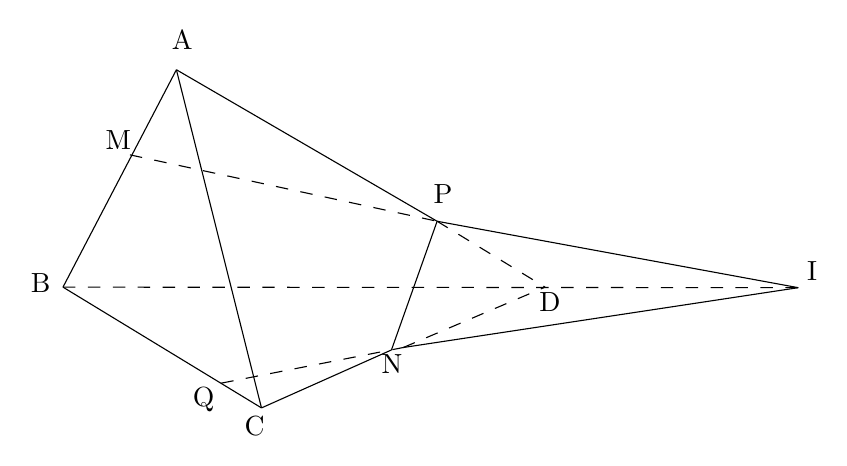
\begin{tikzpicture}[x=0.75pt,y=0.75pt,yscale=-1,xscale=1]
					\draw [dash pattern={on 4.5pt off  4.5pt}] (183.75,137.74) -- (538,138);
					\draw [dash pattern={on  4.5pt off 4.5pt}] (347.69,166.83) -- (416.01,137.74);
					\draw (183.75,137.74) -- (279.38,195.93); 
					\draw (238.39,33) --  (279.38,195.93);
					\draw (238.39,33)  -- (183.75,137.74);
					 \draw (238.39,33) -- (364,106);
					\draw (364,106) -- (342,168); 
					\draw [dash pattern={on 4.5pt off 4.5pt}]  (216,74) -- (364,106);
					\draw  [dash pattern={on 4.5pt off 4.5pt}] (260,184) -- (347.69,166.83);
					\draw (347.69,166.83) -- (538,138); 
					\draw (364,106) -- (538,138); 
					 \draw [dash pattern={on 4.5pt off 4.5pt}] (364,106) -- (416.01,137.74);
					\draw (342,168) -- (279.38,195.93); 
					\draw (541,124) node  [anchor=north west][inner sep=0.75pt] [align=left] {I};
					\draw  (235,13) node [anchor=north west][inner sep=0.75pt] [align=left] {A};
					 \draw (167,130) node [anchor=north west][inner sep=0.75pt] [align=left] {B};
					\draw (203,61) node  [anchor=north west][inner sep=0.75pt] [align=left] {M};
					\draw (361,87) node [anchor=north  west][inner sep=0.75pt] [align=left] {P};
					\draw (412,139) node [anchor=north west][inner sep=0.75pt] [align=left] {D}; 
					\draw (270,199) node [anchor=north west][inner sep=0.75pt] [align=left]  {C};
					\draw (336,169) node [anchor=north west][inner  sep=0.75pt] [align=left] {N};
					\draw (245,185) node [anchor=north west][inner sep=0.75pt]  [align=left] {Q};
				\end{tikzpicture}
		\end{center}
		Ta có:  $ (ABD)\cap (BCD)=BD$.\\
		Mặt  khác: $\heva{
		 {I\in MP,MP\subset (ABD)}\\
		{I\in NQ,NQ\subset  (BCD)}
		 }$\\
		 $\Rightarrow I\in (ABD)\cap (BCD)$.\\
		 Do đó $ I$ thuộc giao tuyến của hai mặt phẳng $ (ABD)$ và $ (BCD)$ hay $ I\in BD$.\\
	Vậy ba điểm $ I,B,D$  thẳng hàng.}
\end{ex}

% nguồn: MaHoaNH_TraLoiNgan_Lop10
\begin{bt}%[0D1V1-2]%[ma:0619bb3b]
	Cho mệnh đề $P:$ \lq\lq $\exists x\in \mathbb{Z}|x^2-4x-5< 0$\rq\rq. Có bao nhiêu giá trị của $x$ để $P$ là mệnh  đề đúng?
	\shortans{5} 
	\loigiai{ 
		Ta  có
		\allowdisplaybreaks 
		\begin{eqnarray*}
			x^2-4x-5< 0 &\Leftrightarrow& \left(x+1\right)\cdot \left(x-5\right) <  0\\
			 &\Leftrightarrow&\hoac{&\heva{&x+1< 0\\&x-5> 0}\\&\heva{&x+1> 0\\&x-5< 0}}\\
			&\Leftrightarrow&\hoac{&x\in \varnothing\\&x\in \left(-1;5\right)}\\ 
			 &\Leftrightarrow&x\in (-1;5)\stackrel{x\in \mathbb{Z}}{\to}x\in \{0;1;2;3;4\}.
		\end{eqnarray*}
		Vậy có  $5$ giá trị thỏa mãn yêu cầu.
	 }
\end{bt}

% nguồn: MaHoaNH_TraLoiNgan_Lop10
\begin{bt}%[0D1V1-2]%[ma:2fba63d4]
	Cho hình vuông $ABCD$ tâm $O$ cạnh bằng  $5$. Gọi $M$ là trung điểm của $AB$, $N$ là điểm đối xứng với $C$ qua $D$. Hãy tính độ dài của vectơ $\overrightarrow{MN}$ (kết quả làm tròn đến hàng phần trăm).
	 \shortans{9,01}
	\loigiai{\begin{center}
		\begin{tikzpicture}[>=stealth,line join=round,line cap=round,font=\footnotesize,scale=0.8]
				\path 
					 (0,4) coordinate (B)
					 (0,0) coordinate (A)
					(4,0) coordinate  (D)
					 (4,4) coordinate (C)
					($(A)!0.5!(C)$) coordinate (O) 
					($(A)!0.5!(B)$) coordinate  (M)
					($(C)!2!(D)$) coordinate  (N);
				\draw  (A)--(B)--(C)--(D)--(A)
					(A)--(C) 
					 (B)--(D)
					(D)--(N)--(M)--(D); 
				\foreach \x/\g in {B/90,A/200,C/30,D/30,O/90,M/160,N/-60} \fill  (\x) circle (1pt) +(\g:3mm) node[scale=.8] {$\x$};
				\draw pic[thin,draw,angle radius=2mm] {right angle=  B--A--D};
				\draw pic[thin,draw,angle radius=2mm] {right  angle= C--B--A};
				\draw pic[thin,draw,angle radius=2mm]  {right angle= D--C--B};
				 \draw pic[thin,draw,angle radius=2mm] {right angle= A--D--C};
			\end{tikzpicture}
	\end{center}
	Áp dụng  định lý Pytago trong tam giác vuông $MAD$ ta có
	$DM^2=AM^2+AD^2=\left(\dfrac{5}{2}\right)^2+5^2=\dfrac{125}{4}$.\\ 
	$\Rightarrow DM=\dfrac{5  \sqrt{5}}{2}$.\\
	Qua  $N$ kẻ đường thẳng song song với $AD$ cắt $AB$ tại $P$.\\
	Khi  đó tứ giác $ADNP$là hình vuông và $PM=PA+AM=5+\dfrac{5}{2}=\dfrac{15}{2}$.\\
	Áp dụng định lý Pytago trong tam giác vuông  $NPM$ ta có
	 $MN^2=NP^2+PM^2=5^2+\left(\dfrac{15}{2}\right)^2=\dfrac{325}{4}$.\\
	 $\Rightarrow MN=\dfrac{5\sqrt{13}}{2}$.\\
	Suy ra $\left|\overrightarrow{MN}\right|=MN=\dfrac{5\sqrt{13}}{2} \approx 9{,}01$. 
 }
\end{bt}


%%%%%%%%%%%%%%%% TỰ LUẬN %%%%%%%%%%%%%%%%

% nguồn: MaHoaNH_TuLuan_Lop10
\begin{bt}%[0D1H1-2]%[ma:21525517]
	Cho mệnh đề $\forall x\in\mathbb{R}$, $x^{2}-5+a>0$  với $a$ là số thực cho trước. Tính tổng các giá trị nguyên của tham số $a<10$ để mệnh đề đã cho là mệnh đề đúng.
	\loigiai{ 
		Mệnh đề $\forall x\in\mathbb{R}$, $x^{2}-5+a>0$ đúng $\Leftrightarrow x^{2}>5-a$  đúng $\forall x\in\mathbb{R}$.\\
		Điều này xảy ra khi  và chỉ khi $\max(5-a) < 0$ đối với $x^2$ (hoặc $5-a$ phải nhỏ hơn $\min(x^2)=0$).\\
		Tức  là $5-a<0\Leftrightarrow a>5$.\\
		Kết hợp với điều kiện $a$ là số nguyên và $a<10$, ta có $a\in\{6; 7; 8; 9\}$.\\ 
		Tổng các giá trị của tham số $a$ là  $6+7+8+9=30$.
	 }
\end{bt}

% nguồn: MaHoaNH_TuLuan_Lop10
\begin{bt}%[0D1H1-2]%[ma:66b19c4f]
	Cho hình thoi $ABCD$ cạnh $2$ và $\widehat{BAD}=60^\circ$.  Tìm độ dài $\overrightarrow{AC}$.
	\loigiai{\begin{center}
		\begin{tikzpicture}[scale=1,line join=round,line cap=round,font=\footnotesize,>=stealth]
				 \def\a{3}
				\def\b{5.25} 
				\path  (0:0) coordinate (B)
					++(0:\a) coordinate (D) 
					([turn]120:\a)  coordinate (A)
					([turn]-150:\b) coordinate  (C)
					($(B)!0.5!(D)$)  coordinate (O);
				\draw (D)--(A)--(B)--(D)--(C)--(B) 
					(A)--(C); 
				\foreach \x/ \goc  in {A/135,B/-135,D/-45,C/-30,O/40}
				\fill (\x) circle (1pt) 
					 ($(\x)+(\goc:3mm)$) node {$\x$};
			\end{tikzpicture}
	\end{center}
	 Gọi $O$ là giao điểm của hai đường chéo $AC$ và $BD$.\\
	Tam giác $ABD$ có $AB=AD$ và $\widehat{BAD}=60^\circ$ nên $\Delta ABD$ đều canh bằng $2$\\ 
	$\Rightarrow  AO=\dfrac{2\sqrt{3}}{2}=\sqrt{3}$.\\
	Khi đó $\left| \overrightarrow{AC}  \right| =AC=2AO=2\sqrt3 \approx 3{,}46$.
 }
\end{bt}

% nguồn: MaHoaNH_TuLuan_Lop10
\begin{bt}%[0D1V1-2]%[ma:9a902021]
	Cho tam giác  $ABC$ đều cạnh $3$ và $G$ là trọng tâm. Gọi $I$ là trung điểm của $AG$. Độ dài của $\overrightarrow{BI}$ là
	\loigiai{\begin{center}
		\begin{tikzpicture}[scale=1,line join=round,line cap=round,font=\footnotesize,>=stealth]
				 \def\a{3}
				\path (0:0)  coordinate (B)
					++(0:\a)  coordinate (C)
					([turn]120:\a) coordinate  (A)
					 ($(B)!0.5!(C)$) coordinate (M)
					($(A)!2/3!(M)$) coordinate  (G)
					($(A)!0.5!(G)$) coordinate (I); 
				 \draw (M)--(A)--(B)--(C)--(A)
					(B)--(I); 
				 \foreach \x/ \goc in {A/135,B/-135,C/-45,M/-90,G/40,I/60}
				\fill (\x)  circle (1pt)
					($(\x)+(\goc:3mm)$) node  {$\x$};
			\end{tikzpicture}
	\end{center}
	Gọi  $M$ là trung điểm của $BC$, nên $BM=\dfrac{3}{2}$\\
	Khi đó $AM$  là đường cao của tam giác $ABC$\\
	 $\Rightarrow AM=\dfrac{3 \sqrt{3}}{2}$.
	Ta  có $\left|\overrightarrow{AG}\right|=AG=\dfrac{2}{3}AM=\dfrac{2}{3} \dfrac{3 \sqrt{3}}{2}=\sqrt{3}$.\\
	Ta có $I$ là trung điểm  của $AG$ nên $MI=AG=\sqrt{3}$.\\
	Xét tam giác $BMI$ vuông tại $M$, ta có\\$\left|\overrightarrow{BI}\right|=BI=\sqrt{B{M^2}+M{I^2}}=\sqrt{\left(\dfrac{3}{2}\right)^2+\left(\sqrt{3}\right)^2}=\dfrac{\sqrt{21}}{2}  \approx 2{,}29$.
} 
\end{bt}

% nguồn: MaHoaNH_TuLuan_Lop10
\begin{bt}%[0D1B1-2]%[ma:05bf9341]
	Xét tính đúng- sai của  các mệnh đề sau
	\begin{enumEX}{1}
		\item $\exists a \in  \mathbb{Q},\, a^2=2$.
		\item $\forall n  \in \mathbb{N}$, $n^2+1$ không chia hết cho $3$.
		 \item $\forall x\in\mathbb{R},\exists y\in\mathbb{R}: x>y\Leftrightarrow x^3>y^3$.
		\item  $\forall x\in\mathbb{R},\forall y\in\mathbb{R}: x+y\geq 2\sqrt{x y}$.
	\end{enumEX}
	\loigiai{\begin{enumEX}{1}
		\item Sai. 
		 \item Đúng.
		\item Đúng. 
		\item Sai. 
\end{enumEX}}
\end{bt}

% nguồn: MaHoaNH_TuLuan_Lop10
\begin{bt}%[0D1B1-2]%[ma:1e4c9bb2]
	Điền vào chỗ trống từ nối \lq\lq và\rq\rq\ hay  \lq\lq hoặc\rq\rq\ để được mệnh đề đúng.
	\begin{listEX}
		\item $\pi <4$  \dots \dots $\pi >5$.
		\item  $ab=0$ khi $a=0$ \dots \dots $b=0$.
		\item $ab\ne 0$ khi $a\ne 0$  \dots \dots $b\ne 0$.
		\item $ab>0$ khi $a>0$ \dots \dots  $b>0$ \dots \dots $a<0$ \dots \dots $b<0$.
		\item Một số chia hết cho $6$ khi và  chỉ khi nó chia hết cho $2$ \dots \dots cho $3$.
		\item Một số chia hết cho $5$ khi và chỉ khi chữ số tận cùng của nó bằng $0$ \dots \dots  bằng $5$.
	\end{listEX}
	 \loigiai{
		\begin{listEX}
			\item  $\pi <4$ hoặc $\pi >5$.
			\item $ab=0$ khi $a=0$ hoặc $b=0$. 
			\item $ab\ne  0$ khi $a\ne 0$ và $b\ne 0$.
			\item  $ab>0$ khi $a>0$ và $b>0$ hoặc $a<0$ và $b<0$.
			\item Một  số chia hết cho $6$ khi và chỉ khi nó chia hết cho $2$ và cho $3$.
			\item Một số chia hết cho $5$ khi và chỉ khi chữ số tận cùng của nó bằng $0$ hoặc bằng $5$. 
		\end{listEX}
	 }
\end{bt}

% nguồn: MaHoaNH_TuLuan_Lop10
\begin{bt}%[0D1B1-2]%[ma:78c750d1]
	Trong các câu sau, câu nào là mệnh đề, câu nào không là mệnh đề? Nếu là mệnh đề thì nó là mệnh đề đúng hay  sai?
	\begin{listEX}
		\item Các em  có vui không?
		\item Cấm học sinh nói  chuyện trong giờ học!
		\item Phương trình $x^2+x=0$ có hai nghiệm  dương phân biệt.
		\item  $2^5-1$ là một số nguyên tố.
		\item $\sqrt{2}$ là một số vô  tỉ.
		\item Thành phố Hồ Chí Minh  là thủ đô của nước Việt Nam.
		\item Một số tự nhiên chia hết cho $2$ và  $4$ thì số đó chia hết cho $8$.
	\end{listEX}
	\loigiai{ 
		\begin{listEX}
			\item Các em có vui không? Câu này không là  mệnh đề.
			\item Cấm học sinh nói chuyện trong giờ học! Câu này không là mệnh đề. 
			\item Phương trình $x^2+x=0$ có  hai nghiệm dương phân biệt. Câu này là mệnh đề sai.
			\item $2^5-1$ là một  số nguyên tố. Câu này là mệnh đề đúng.
			\item $\sqrt{2}$ là một số  vô tỉ. Câu này là mệnh đề đúng.
			\item Thành phố  Hồ Chí Minh là thủ đô của nước Việt Nam. Câu này là mệnh đề sai.
			\item Một số tự  nhiên chia hết cho $2$ và $4$ thì số đó chia hết cho $8$. Câu này là mệnh đề sai.
		\end{listEX}
	 }
\end{bt}

% nguồn: MaHoaNH_TuLuan_Lop10
\begin{bt}%[0D1B1-2]%[ma:e4e816fd]
	Trong các mệnh đề sau,  mệnh đề nào đúng? Giải thích?
	\begin{listEX}
		\item Hai tam giác bằng nhau khi và chỉ khi  chúng có diện tích bằng nhau.
		\item Hai tam giác bằng  nhau khi và chỉ khi chúng đồng dạng và có một cạnh bằng nhau.
		\item Một tam giác là tam giác đều khi và chỉ khi chúng có hai đường trung tuyến bằng nhau và có một góc  bằng $60^\circ$.
		\item Một tam giác là tam giác vuông khi và  chỉ khi nó có một góc bằng tổng của hai góc còn lại.
		\item Đường tròn có một  tâm đối xứng và một trục đối xứng.
		\item  Hình chữ nhật có hai trục đối xứng.
		\item Một tứ giác là hình thoi khi và chỉ khi nó có hai  đường chéo vuông góc với nhau.
		\item Một tứ giác nội tiếp  được đường tròn khi và chỉ khi nó có hai góc vuông.
	\end{listEX}
	\loigiai{ 
		\begin{listEX}
			\item Hai tam giác bằng nhau khi và chỉ khi chúng có diện tích bằng nhau. Mệnh đề sai vì một tam giác có chiều cao $3$ cm, cạnh đáy tương ứng $4$ cm cùng diện tích với tam giác có chiều cao $6$ cm, cạnh đáy tương ứng $2$ cm. Nhưng hai  tam giác này không bằng nhau vì không có ba cặp cạnh và ba cặp góc bằng nhau.
			\item Hai tam giác bằng nhau khi và chỉ khi chúng đồng dạng và có một cạnh bằng nhau. Mệnh đề sai vì một tam giác có số đo ba cạnh $3$ cm, $4$ cm, $6$ cm đồng dạng với tam giác có số đó ba cạnh $6$ cm, $8$ cm, $12$ cm nhưng chúng không bằng  nhau.
			\item Một tam giác là tam giác đều khi và chỉ khi chúng có hai đường trung tuyến bằng nhau và có một góc bằng $60^\circ$. Mệnh đề đúng vì tam giác có hai đường trung  tuyến bằng nhau là tam giác cân và có thêm một góc bằng $60^\circ$ thì trở thành tam giác đều.
			\item Một tam giác là tam giác vuông khi và chỉ  khi nó có một góc bằng tổng của hai góc còn lại. Mệnh đề đúng, dùng kiến thức tổng ba góc trong một tam giác để chứng minh.
			\item Đường tròn có một tâm đối xứng và một trục đối xứng. Mệnh đề sai vì đường tròn có một tâm  đối xứng nhưng có vô số trục đối xứng.
			\item Hình chữ nhật  có hai trục đối xứng. Mệnh đề đúng.
			\item Một tứ giác là hình thoi khi và chỉ khi nó có hai đường chéo vuông góc với nhau. Mệnh đề sai vì một tứ giác  là hình thoi khi và chỉ khi nó là hình bình hành và có hai đường chéo vuông góc với nhau.
			\item Một tứ giác nội tiếp được đường tròn khi và chỉ khi nó có hai góc vuông. Mệnh đề  sai, ví dụ là hình thang vuông.
		\end{listEX}
	 }
\end{bt}

% nguồn: MaHoaNH_TuLuan_Lop10
\begin{bt}%[0D1B1-2]%[ma:df20db3d]
	Trong các mệnh đề sau, mệnh đề nào  đúng? Giải thích?
	\begin{enumEX}{2}
		\item Nếu $a$ chia hết cho $9$ thì $a$  chia hết cho $3$.
		\item Nếu $a\ge  b$ thì $a^2\ge b^2$.
		\item Nếu $a$ chia hết cho $3$ thì $a$ chia hết  cho $6$.
		 \item Số $\pi$ lớn hơn $2$ và nhỏ hơn $4$.
		\item $2$  và $3$ là hai số nguyên tố cùng nhau.
		 \item $81$ là một số chính phương.
		\item $5>3$  hoặc $5<3$.
		\item Số $15$ chia hết cho $4$ hoặc cho $5$. 
	\end{enumEX}
	 \loigiai{
		\begin{enumEX}{1}
			\item Nếu $a$ chia hết cho $9$ thì $a$ chia hết cho $3$. Mệnh đề đúng vì $a\vdots 9$ thì $a$ được biểu  diễn $a=9b=3\cdot 3b$ ($b\in \mathbb{Z}$), suy ra $a\vdots 3$.
			\item Nếu $a\ge b$ thì $a^2\ge b^2$. Mệnh đề  sai vì $1\ge -2$ nhưng $(1)^2\le (-2)^2$.
			\item Nếu $a$ chia hết cho $3$  thì $a$ chia hết cho $6$. Mệnh đề sai vì $9$ chia hết cho $3$ nhưng không chia hết cho $6$.
			\item Số $\pi$ lớn hơn $2$ và nhỏ hơn $4$. Mệnh  đề đúng vì $\pi \approx 3{,}14$.
			\item $2$ và $3$ là hai số nguyên tố cùng  nhau. Mệnh đề đúng vì chúng có ước chung lớn nhất bằng $1$.
			\item $81$ là một số chính  phương. Mệnh đề đúng vì $81=9^2$.
			\item $5>3$ hoặc $5<3$. Mệnh đề đúng vì mệnh đề $A$ hoặc $B$ đúng khi $A$ đúng hoặc  $B$ đúng.
			\item Số $15$  chia hết cho $4$ hoặc cho $5$. Mệnh đề đúng vì $15$ chia hết cho $5$.
		\end{enumEX}
	 }
\end{bt}

% nguồn: MaHoaNH_TuLuan_Lop10
\begin{bt}%[0D1B1-2]%[0D1B1-3]%[ma:41c797dc]
	Xét tính đúng, sai và lập mệnh đề phủ định của  mỗi mệnh đề sau:
	\begin{enumEX}{1}
		\item $\exists n\in\mathbb{N}\colon 7n^2$  chia hết cho $n$.
		\item $\exists x\in\mathbb{R}\colon x^2-6x+10>0$. 
		\item $\forall x\in\mathbb{Q}\colon x^2-9\ne 9x$. 
		\item Tổng hai góc nhọn của một tam giác vuông bằng $90^\circ$. 
		\item $\sqrt{4}$ là  số vô tỉ.
		\item Berlin là  thủ đô của nước Đức.
	\end{enumEX}
	\loigiai{ 
		\begin{enumEX}{1}
			\item Khi $n=1$ thì $7\cdot 1^2$ chia hết cho $1$, nên mệnh đề \lq\lq$\exists n\in\mathbb{N}\colon 7n^2$ chia hết cho $n$\rq\rq\, là mệnh đề đúng.\\ 
			Mệnh đề phủ định của nó là: \lq\lq$\forall n\in\mathbb{N}\colon 7n^2$ không chia  hết cho $n$.\rq\rq
			\item Khi $x=0$ ta có $0^2-6\cdot 0+10=10>0$ nên mệnh đề \lq\lq$\exists x\in\mathbb{R}\colon x^2-6x+10>0$\rq\rq\,  là mệnh đề đúng.\\
			 Mệnh đề phủ định của nó là: \lq\lq$\forall x\in\mathbb{R}\colon x^2-6x+10\le 0$\rq\rq.
			\item Ta có $x^2-9= 9x \Leftrightarrow x=\dfrac{9\pm 3\sqrt{13}}{2}\notin \mathbb{Q}$ nên mệnh đề \lq\lq$\forall x\in\mathbb{Q}\colon x^2-7\ne 7x$\rq\rq\, là mệnh  đề đúng.\\
			Mệnh đề  phủ định của nó là: \lq\lq$\exists x\in\mathbb{Q}\colon x^2-9= 9x$\rq\rq.
			\item Mệnh đề \lq\lq Tổng hai góc  nhọn của một tam giác vuông bằng $90^\circ$\rq\rq \, là mệnh đề đúng.\\
			Mệnh đề phủ định của nó là: \lq\lq  Tổng hai góc nhọn của một tam giác vuông không bằng $90^\circ$\rq\rq.
			\item Mệnh đề \lq\lq $\sqrt{4}$ là số vô tỉ\rq\rq \, là mệnh đề sai.\\ 
			Mệnh đề phủ định của  nó là: \lq\lq $\sqrt{4}$ là số hữu tỉ\rq\rq.
			\item Mệnh đề \lq\lq Berlin là thủ  đô của nước Đức\rq\rq \, là mệnh đề đúng.\\
			Mệnh đề phủ định của nó là: \lq\lq Berlin không phải là thủ  đô của nước Đức\rq\rq.
	\end{enumEX}}
\end{bt}

% nguồn: MaHoaNH_TuLuan_Lop10
\begin{bt}%[0D1B1-2]%[0D1B1-3]%[ma:a6b4677f]
	Xét tính đúng, sai và lập mệnh đề phủ  định của mỗi mệnh đề sau:
	\begin{enumEX}{1}
		\item  $\forall n\in\mathbb{N}\colon 4n^2$ chia hết cho $n$.
		\item $\forall x\in\mathbb{R}\colon x^2-6x+10>0$. 
		\item $\exists x\in\mathbb{Q}\colon x^2-7\ne  7x$.
		\item Tổng ba góc trong của  một tam giác bằng $180^\circ$.
		\item  $\sqrt{9}$ là số vô tỉ.
		\item Paris là thủ  đô của nước Pháp.
	\end{enumEX}
	\loigiai{ 
		\begin{enumEX}{1}
			\item Ta có $4n^2:n=4n$ nên mệnh đề \lq\lq$\forall n\in\mathbb{N}\colon 4n^2$ chia hết cho $n$\rq\rq\, là mệnh đề  đúng.\\
			Mệnh đề phủ định của nó là: \lq\lq$\exists n\in\mathbb{N}\colon 4n^2$ không chia hết cho  $n$\rq\rq.
			\item Ta có $x^2-6x+10=(x-3)^2+1>0, \forall x\in\mathbb{R}$ nên mệnh đề \lq\lq$\forall x\in\mathbb{R}\colon x^2-6x+10>0$\rq\rq\, là mệnh  đề đúng.\\
			Mệnh đề phủ định  của nó là: \lq\lq$\exists x\in\mathbb{R}\colon x^2-6x+10\le 0$\rq\rq.
			\item Với $x=0\in\mathbb{Q}$ ta có $0^2-7\ne 7\cdot 0$ nên mệnh đề \lq\lq$\exists x\in\mathbb{Q}\colon  x^2-7\ne 7x$\rq\rq\, là mệnh đề đúng.\\
			Mệnh  đề phủ định của nó là: \lq\lq$\forall x\in\mathbb{Q}\colon x^2-7= 7x$\rq\rq.
			 \item Mệnh đề \lq\lq Tổng ba góc trong của một tam giác bằng $180^\circ$\rq\rq \, là mệnh đề đúng.\\
			Mệnh đề phủ định  của nó là: \lq\lq Tổng ba góc trong của một tam giác không bằng $180^\circ$\rq\rq.
			\item Mệnh đề \lq\lq  $\sqrt{9}$ là số vô tỉ\rq\rq \, là mệnh đề sai.\\
			Mệnh đề phủ định của nó là: \lq\lq $\sqrt{9}$ là số hữu tỉ\rq\rq. 
			\item Mệnh đề \lq\lq Paris là thủ đô của  nước Pháp\rq\rq \, là mệnh đề đúng.\\
			Mệnh đề phủ định của nó là: \lq\lq Paris không phải là  thủ đô của nước Pháp\rq\rq.
	\end{enumEX}}
\end{bt}

% nguồn: MaHoaNH_TuLuan_Lop10
\begin{bt}%[0D1K1-2]%[ma:c3de65c9]
	Cho mệnh đề  chứa biến $P(x)$, với $x\in \mathbb{R}$. Tìm $x$ để $P(x)$ là mệnh đề đúng.
	\begin{enumEX}{2}
		\item $P(x):\text{\lq\lq}  x^2-5x+4=0\text{\rq\rq}$.
		\item $P(x):\text{\lq\lq} x^2-5x+6=0\text{\rq\rq}$. 
		\item  $P(x):\text{\lq\lq} x^2-3x>0\text{\rq\rq}$.
		 \item $P(x):\text{\lq\lq} \sqrt{x}\ge x\text{\rq\rq}$.
		 \item $P(x):\text{\lq\lq} 2x+3\le 7\text{\rq\rq}$.
		 \item $P(x):\text{\lq\lq} x^2+x+1>0\text{\rq\rq}$.
	\end{enumEX}
	 \loigiai{
		\begin{enumEX}{1}
			\item  $P(x):\text{\lq\lq} x^2-5x+4=0\text{\rq\rq}$.\\
			$x^2-5x+4=0\Leftrightarrow x=1\text{  hoặc }x=4$.\\
			 Vậy $x=1\text{ hoặc }x=4$ thì $P(x)$ đúng.
			\item  $P(x):\text{\lq\lq} x^2-5x+6=0\text{\rq\rq}$.\\
			$x^2-5x+6=0\Leftrightarrow x=2\text{  hoặc }x=3$.\\
			Vậy  $x=2\text{ hoặc }x=3$ thì $P(x)$ đúng.
			\item  $P(x):\text{\lq\lq} x^2-3x>0\text{\rq\rq}$.\\
			$x^2-3x>0\Leftrightarrow x(x-3)>0\Leftrightarrow \heva{&x>0\\&x-3>0}\text{ hoặc }\heva{&x<0\\&x-3<0}\Leftrightarrow x>3\text{  hoặc }x<0$.\\
			Vậy $x>3\text{ hoặc  }x<0$ thì $P(x)$ đúng.
			 \item $P(x):\text{\lq\lq} \sqrt{x}\ge x\text{\rq\rq}$.\\
			$\sqrt{x}\ge x\Leftrightarrow \heva{&x\ge 0\\&x\ge x^2}\Leftrightarrow \heva{&x\ge 0\\&x(x-1)\le 0}\Leftrightarrow  \heva{&x\ge 0\\&x-1\le 0}\Leftrightarrow 0\le x\le 1$.\\
			Vậy $0\le x\le  1$ thì $P(x)$ đúng.
			\item  $P(x):\text{\lq\lq} 2x+3\le 7\text{\rq\rq}$.\\
			$2x+3\le  7\Leftrightarrow x\le 2$.\\
			Vậy $x\le 2$ thì $P(x)$  đúng.
			\item $P(x):\text{\lq\lq} x^2+x+1>0\text{\rq\rq}$.\\ 
			 Ta có $x^2+x+1=\left( x+\dfrac{1}{2}\right)^2+\dfrac{3}{4}>0$, $\forall x\in \mathbb{R}$.\\
			Vậy $P(x)$ đúng  với mọi $x\in \mathbb{R}$.
		\end{enumEX}
	 }
\end{bt}
